\documentclass{article}
\usepackage{graphicx}
\usepackage{wrapfig}
\usepackage{subcaption}
\usepackage[margin=1in]{geometry}
\usepackage{amsmath} % or simply amstext
\usepackage{siunitx}
\usepackage{booktabs}
\usepackage[export]{adjustbox}
\newcommand{\angstrom}{\textup{\AA}}
\usepackage{cleveref}
\usepackage{booktabs}
\usepackage{gensymb}
\usepackage{float}

\title{Supplmental Information : Understanding the nanoscale structure of hexagonal phase lyotropic liquid crystal membranes}
\author{Benjamin J. Coscia \and Douglas L. Gin \and Richard D. Noble \and Joe Yelk \and Matthew Glaser \and Xunda Feng \and Michael R. Shirts}

\begin{document}

  \bibliographystyle{ieeetr}
  \graphicspath{{./figures/}}  % put all the figures here
  \maketitle

  \noindent
  \begingroup
	\fontsize{14pt}{14pt}\selectfont
	\textbf{Further details regarding monomer parameterization} 
  \endgroup
 
  \vspace{1em}
  We parameterized monomers according to the following procedure:
  \begin{enumerate}
	\item \textit{Create monomer structure file with connectivity} : We
	drew atomistic structures using MarvinSketch
	17.13~\cite{chemaxon_marvinsketch_2017} with all hydrogen atoms drawn out
	explicitly. We optimized the 3D geometry of the structure using the 'Clean in
	3D' function of MarvinSketch.  We saved the structure as a .mol file, then
	converted it to .pdb format using Open Babel 2.4.1
	\cite{oboyle_open_2011,noauthor_open_nodate}. 
	\item \textit{Assign GAFF atomtypes using \texttt{antechamber}} : Using
	the .pdb structure file as input, we ran
	\texttt{antechamber}~\cite{wang_automatic_2006} using the AM1-BCC charge model.
	The net charge on the monomer is input as -1 since the sodium ion is kept as 
	a separate residue. We use \texttt{LEaP}~\cite{case_ambertools16_2016} and the
	output of \texttt{antechamber} to create Amber topology files. A detailed
	tutorial can be accessed elsewhere \cite{walker_antechamber_nodate}.
	\item \textit{Create GROMACS topologies from Amber output} : The output
	of \texttt{LEaP} is a .inpcrd and a .prmtop file which are Amber topology
	files. Using acpype.py \cite{sousa_da_silva_acpype_2012}, we converted the
	\texttt{LEaP} output into GROMACS .gro and .top files. 
	\item \textit{Perform a simulated annealing procedure on the monomer} :
	We created a cubic box around the monomer using the GROMACS command \texttt{gmx
	editconf}. The monomer was centered in the box with edges of the
	box spaced at least 3 nm from the monomer on all sides. We ran an energy minimzation
	on the system with the steepest descent algorithm. Next we performed an NVT
	simulated annealing procedure. We linearly decreased the temperature of the
	system from 1000 K to 50 K over the course of 10 ns. We randomly chose a monomer
	configuration from the last 10 \% of the trajectory. 
	\item \textit{Reassign charges with \texttt{molcharge}}: With the monomer
	configuration taken from the annealed trajectory, we reassigned charges using
	\texttt{molcharge} with the am1bccsym method in order to ensure charges 
	are symmetric. This condition is not guaranteed with \texttt{antechamber}. 
	The charges in the GROMACS topology file (.top) were replaced with the 
	new charges calculated by \texttt{molcharge}. 
	\item \textit{Anneal again to get final structure} : We repeated the
	same simulated annealing procedure using the monomer topology with
	\texttt{molcharge} charges. A random monomer configuration was pulled from the
	last 10 \% of the trajectory and was used to build all assemblies reported
	(Figure~\ref{fig:monomer}).
  \end{enumerate} 

  \begin{figure}
	\centering
        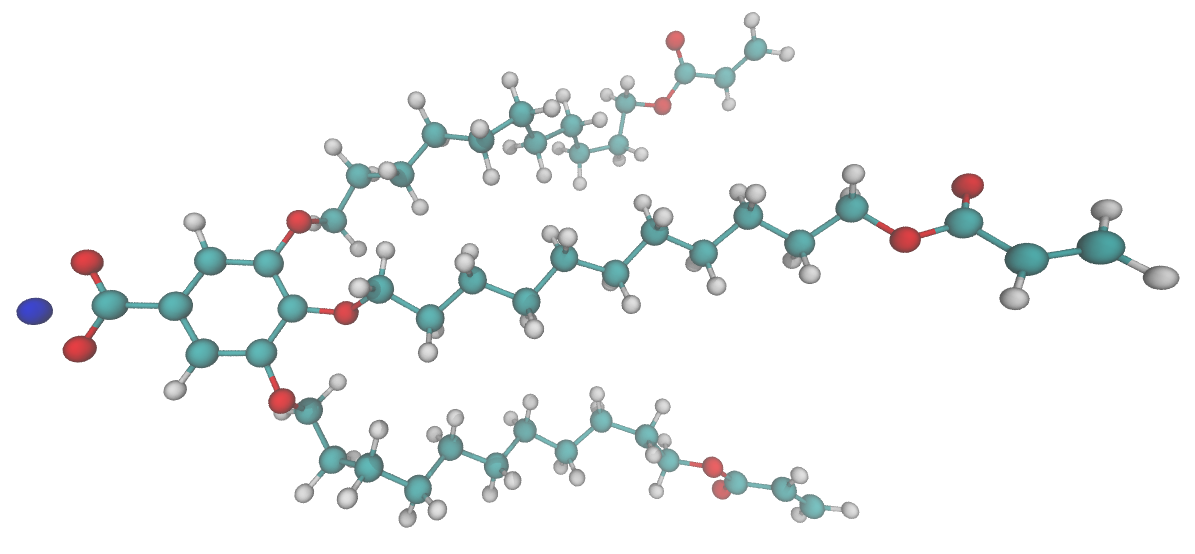
\includegraphics[width=0.9\textwidth]{monomer.png}
	\caption{Atomistic representation of the monomer Na-GA3C11. White atoms
		represent hydrogen, cyan atoms represent carbon, red atoms represent oxygen and
		the blue atom is sodium.}\label{fig:monomer}
  \end{figure}

  \begin{figure}
	\centering
        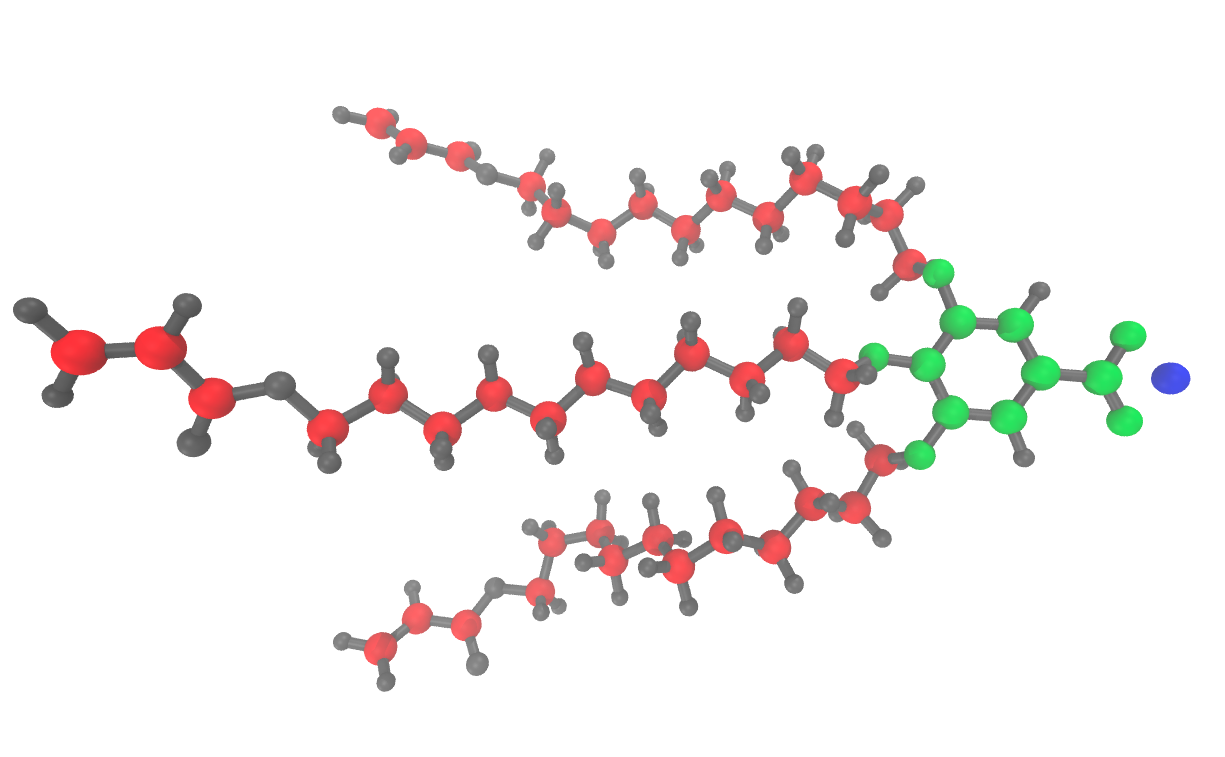
\includegraphics[width=0.9\textwidth]{monomer_color_coded.png}
	\caption{The groups used for $g(z)$ calculations. Red atoms are in the
		tails group. Green atoms are in the head group region. The blue atom is sodium. 
		}\label{fig:monomer_color_coded}
  \end{figure}

  \begin{figure}
        \centering
        \begin{subfigure}[b]{0.32\textwidth}
                \centering
                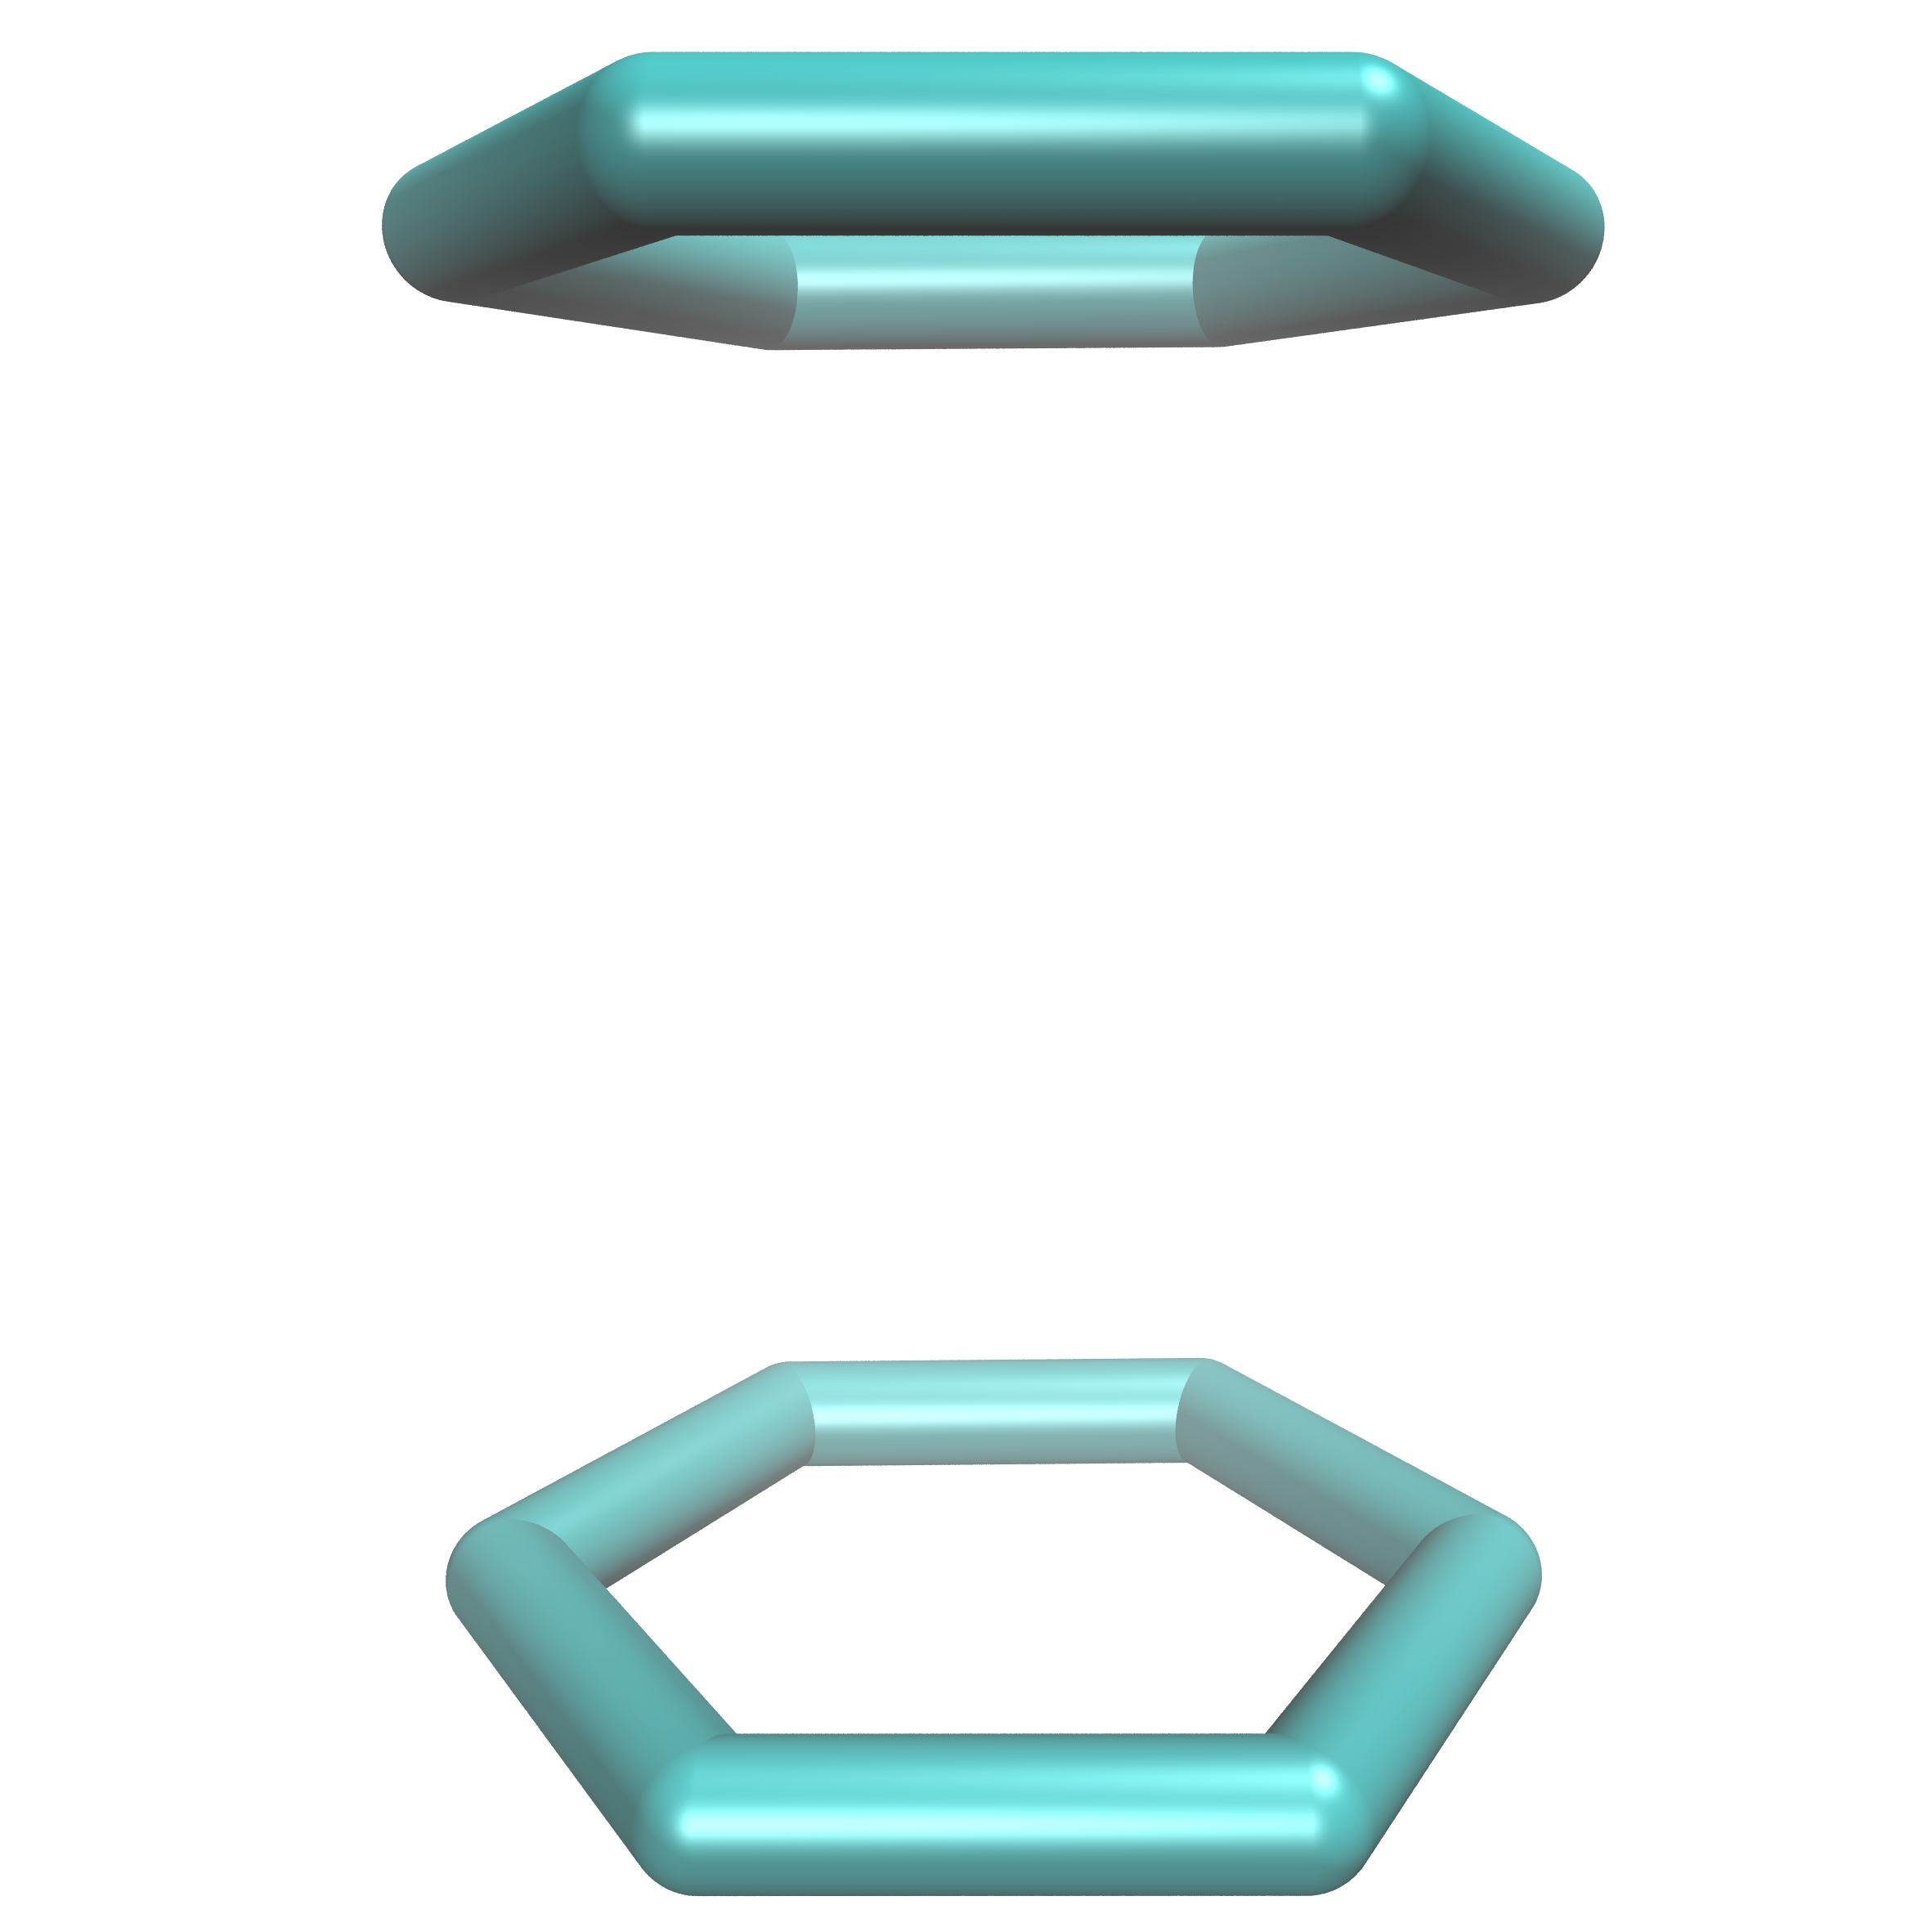
\includegraphics[width=\textwidth]{sandwiched.png}
                \caption{}\label{fig:sandwiched}
        \end{subfigure}
        \begin{subfigure}[b]{0.32\textwidth}
                \centering
                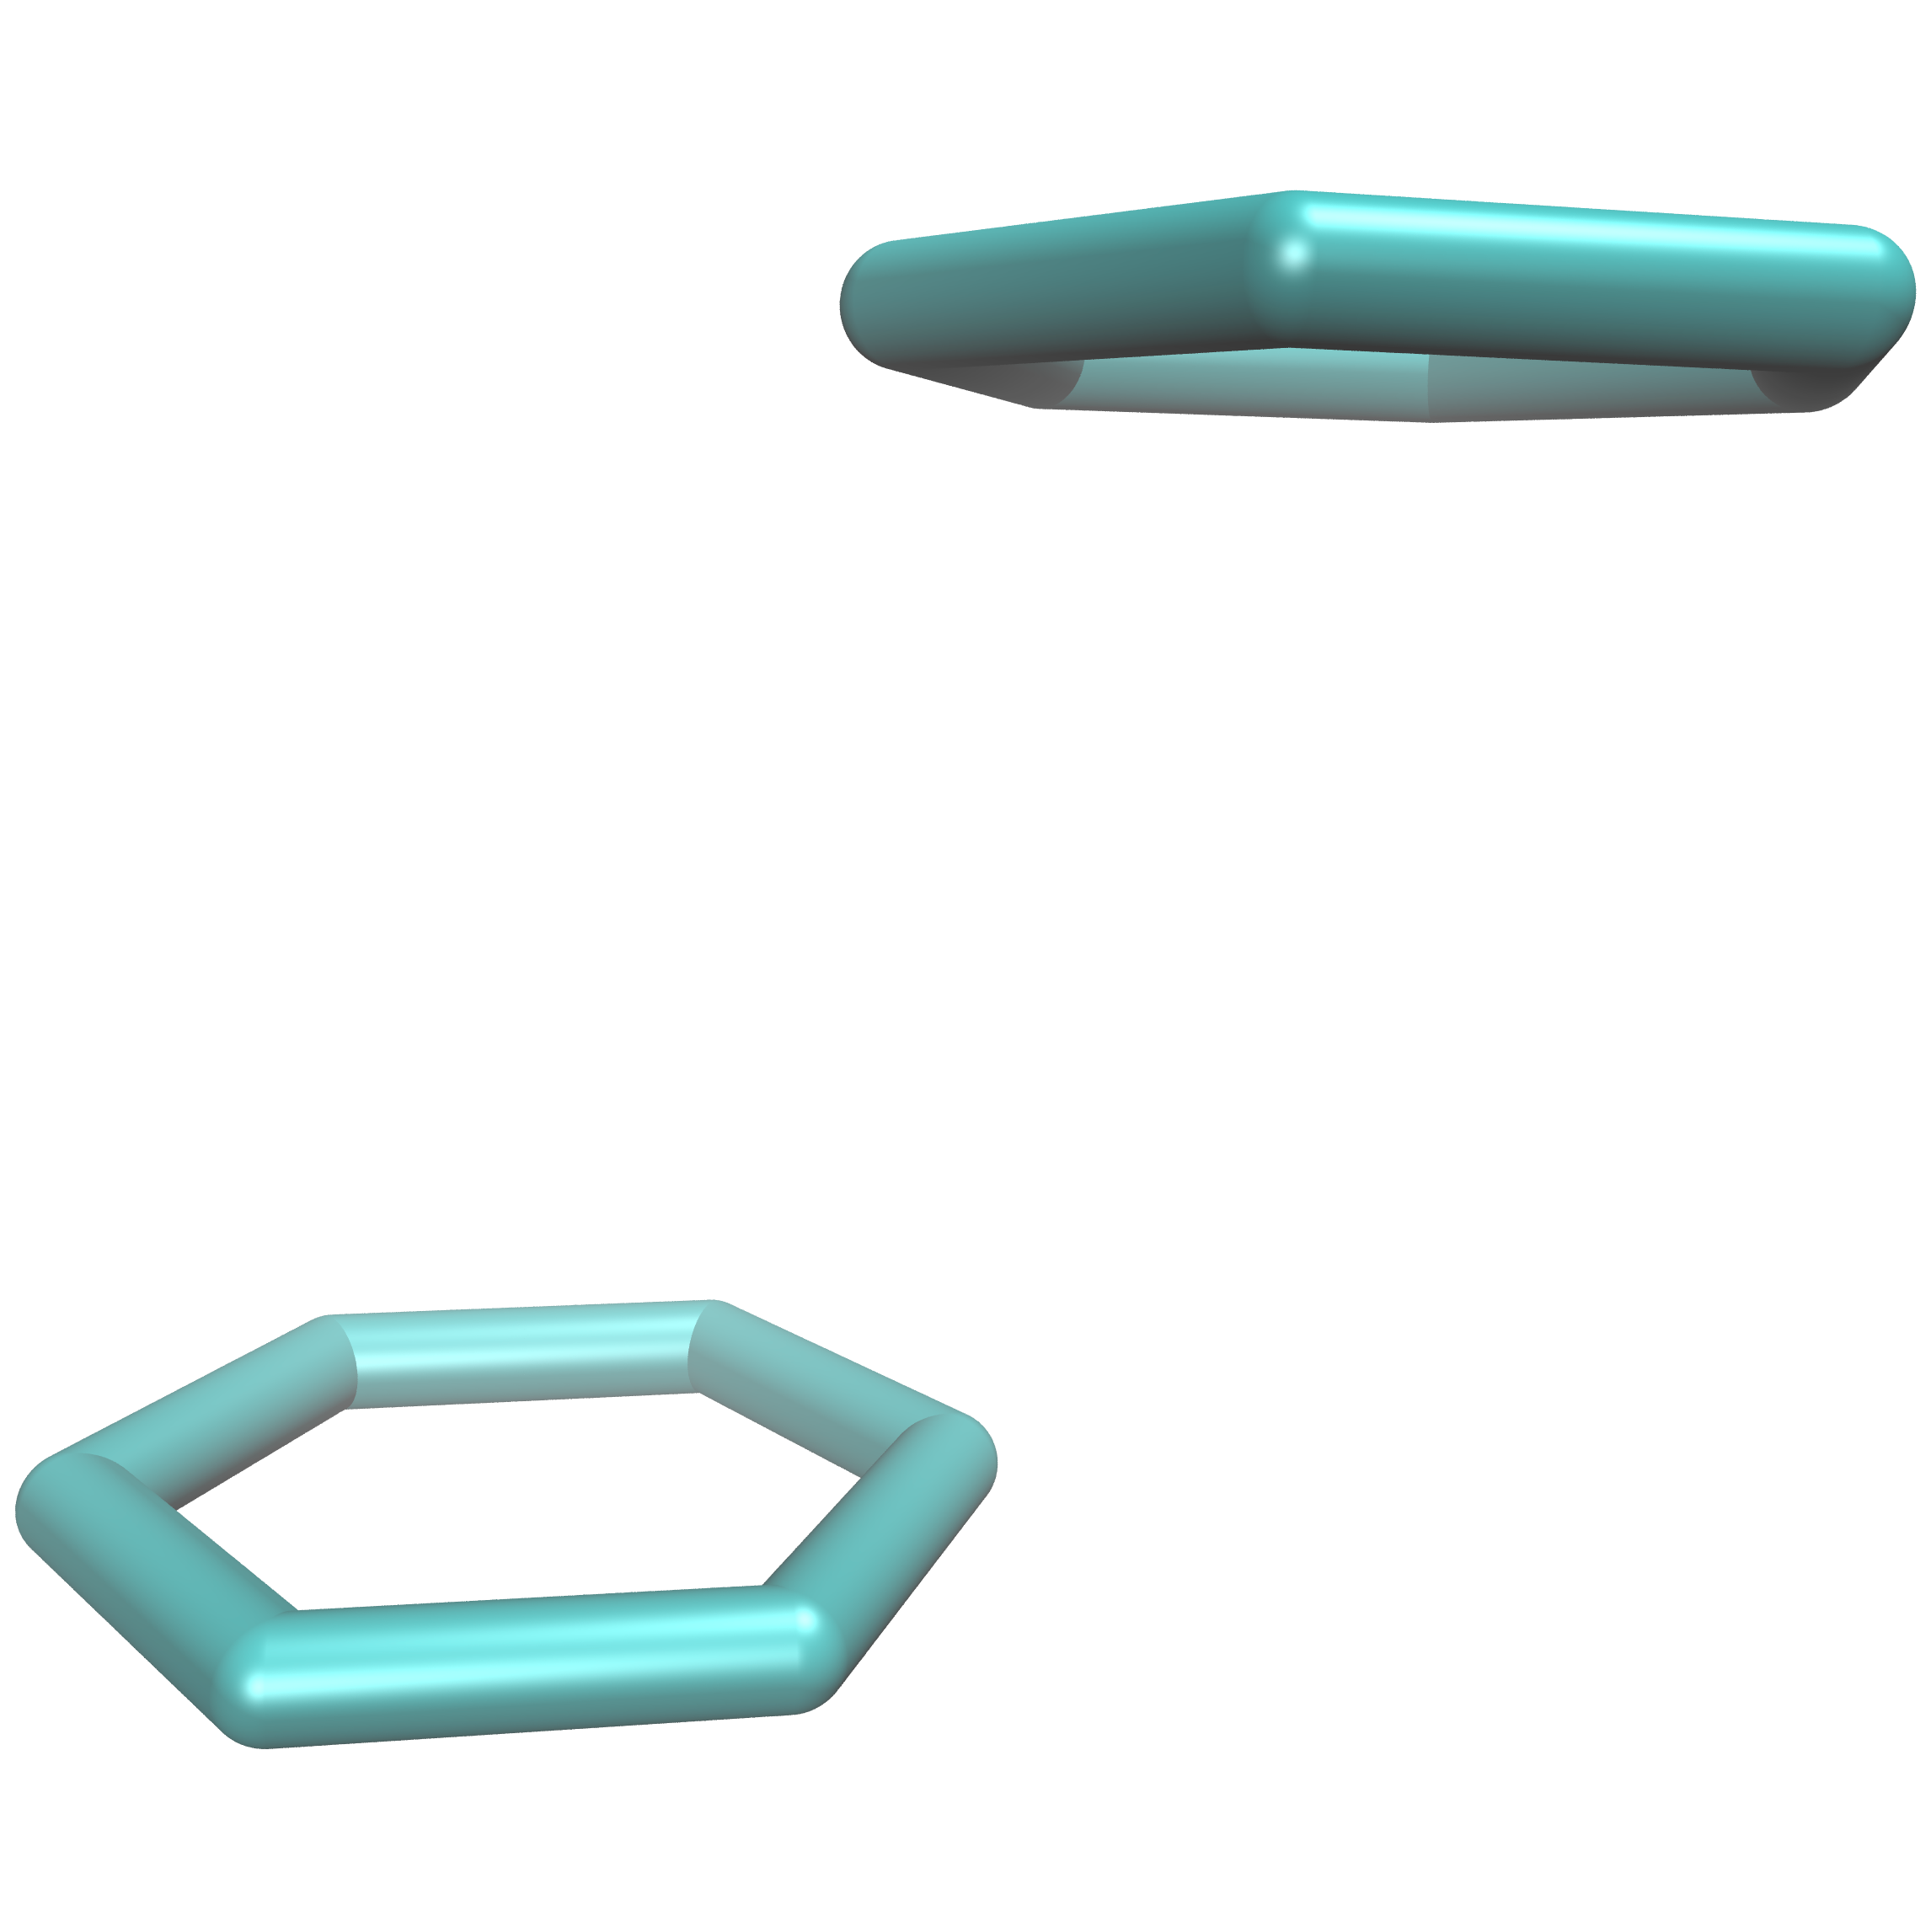
\includegraphics[width=\textwidth]{PD.png}
                \caption{}\label{fig:pd}
        \end{subfigure}
        \begin{subfigure}[b]{0.32\textwidth}
                \centering
                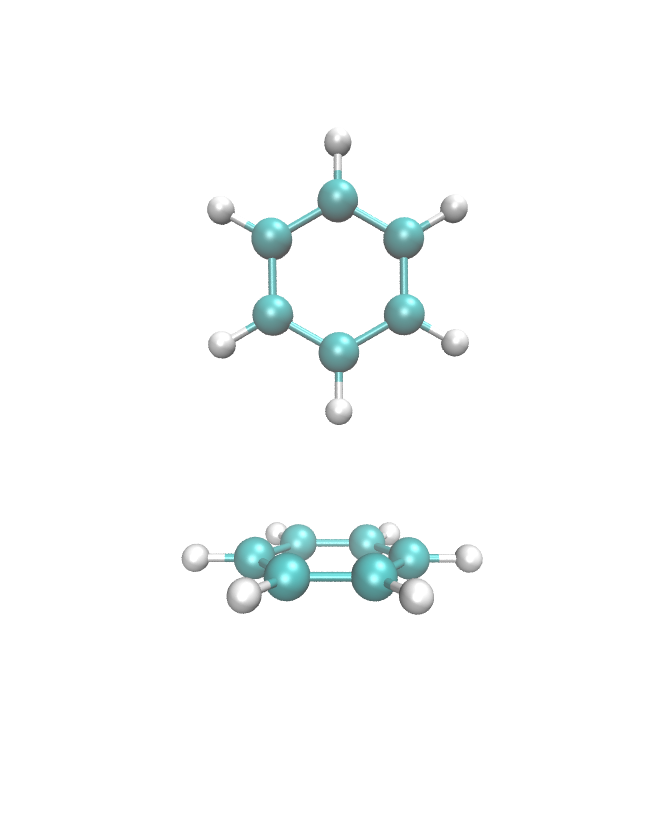
\includegraphics[width=\textwidth]{Tshaped.png}
                \caption{}\label{fig:tshaped}
        \end{subfigure}
        \vskip\baselineskip
        \begin{subfigure}[b]{0.475\textwidth}
                \centering
                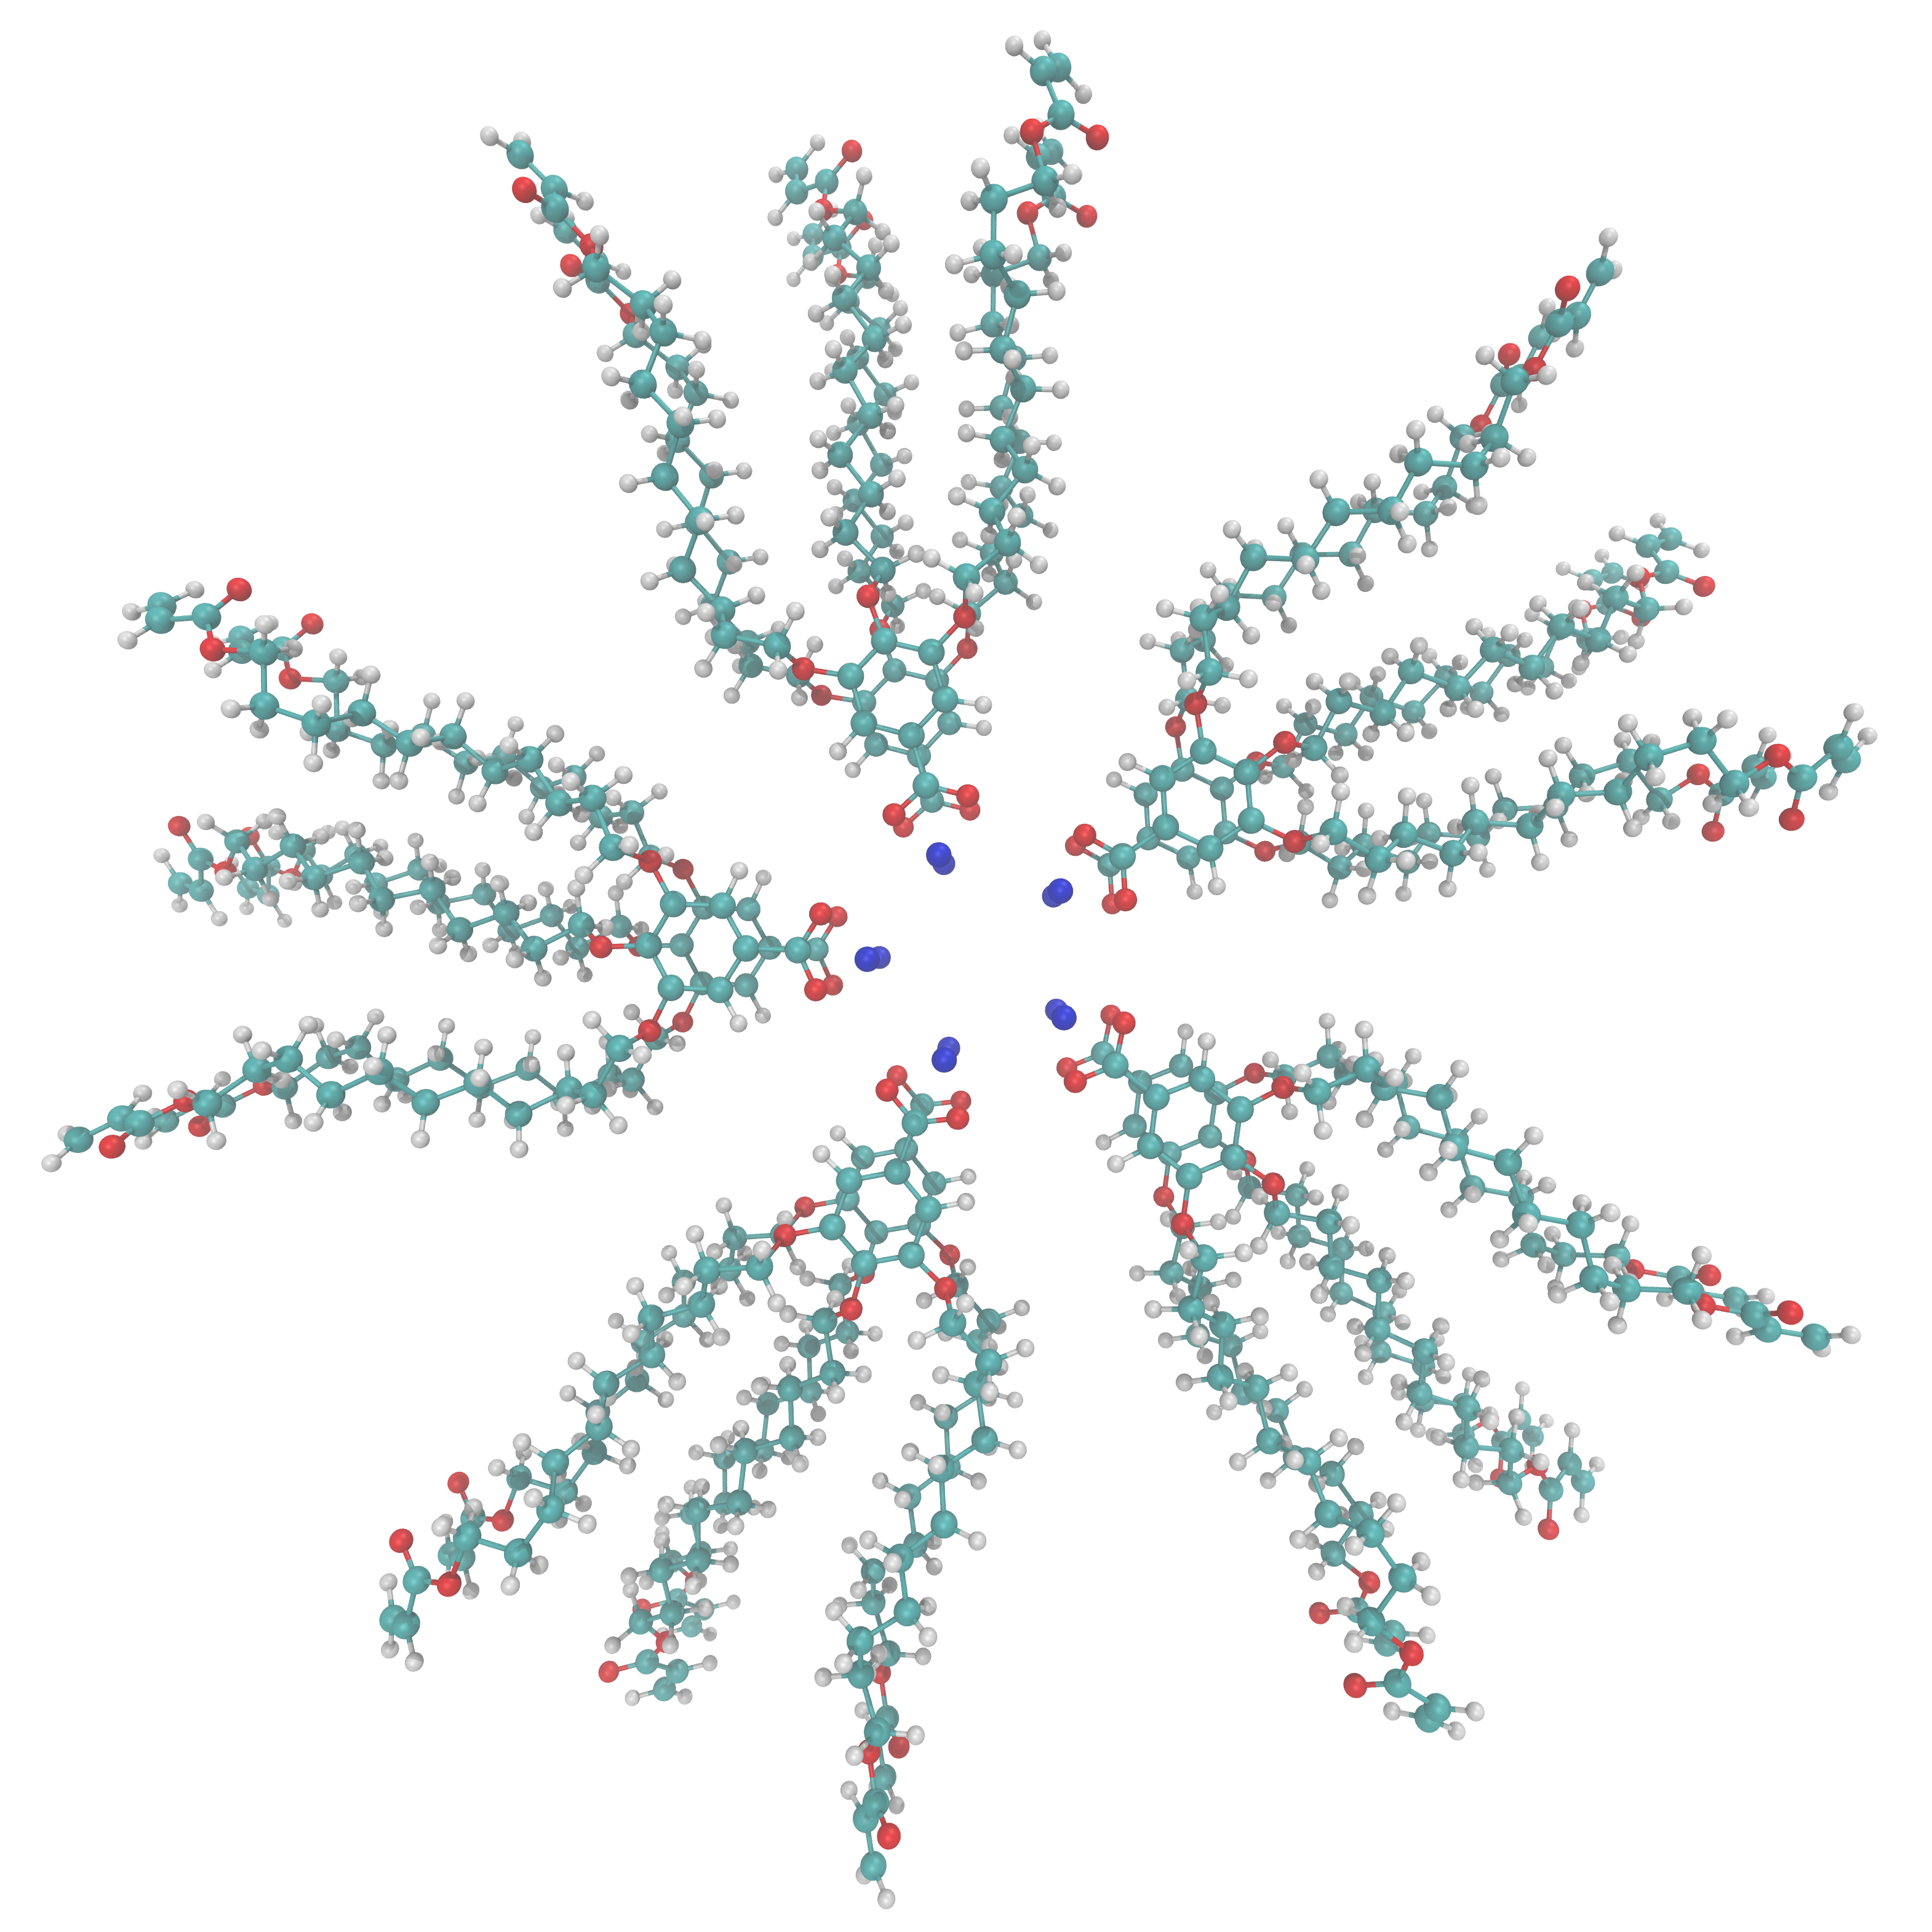
\includegraphics[width=\textwidth]{sandwichedlayers.png}
                \caption{}\label{fig:sandwichedlayers}
        \end{subfigure}
        \begin{subfigure}[b]{0.475\textwidth}
                \centering
                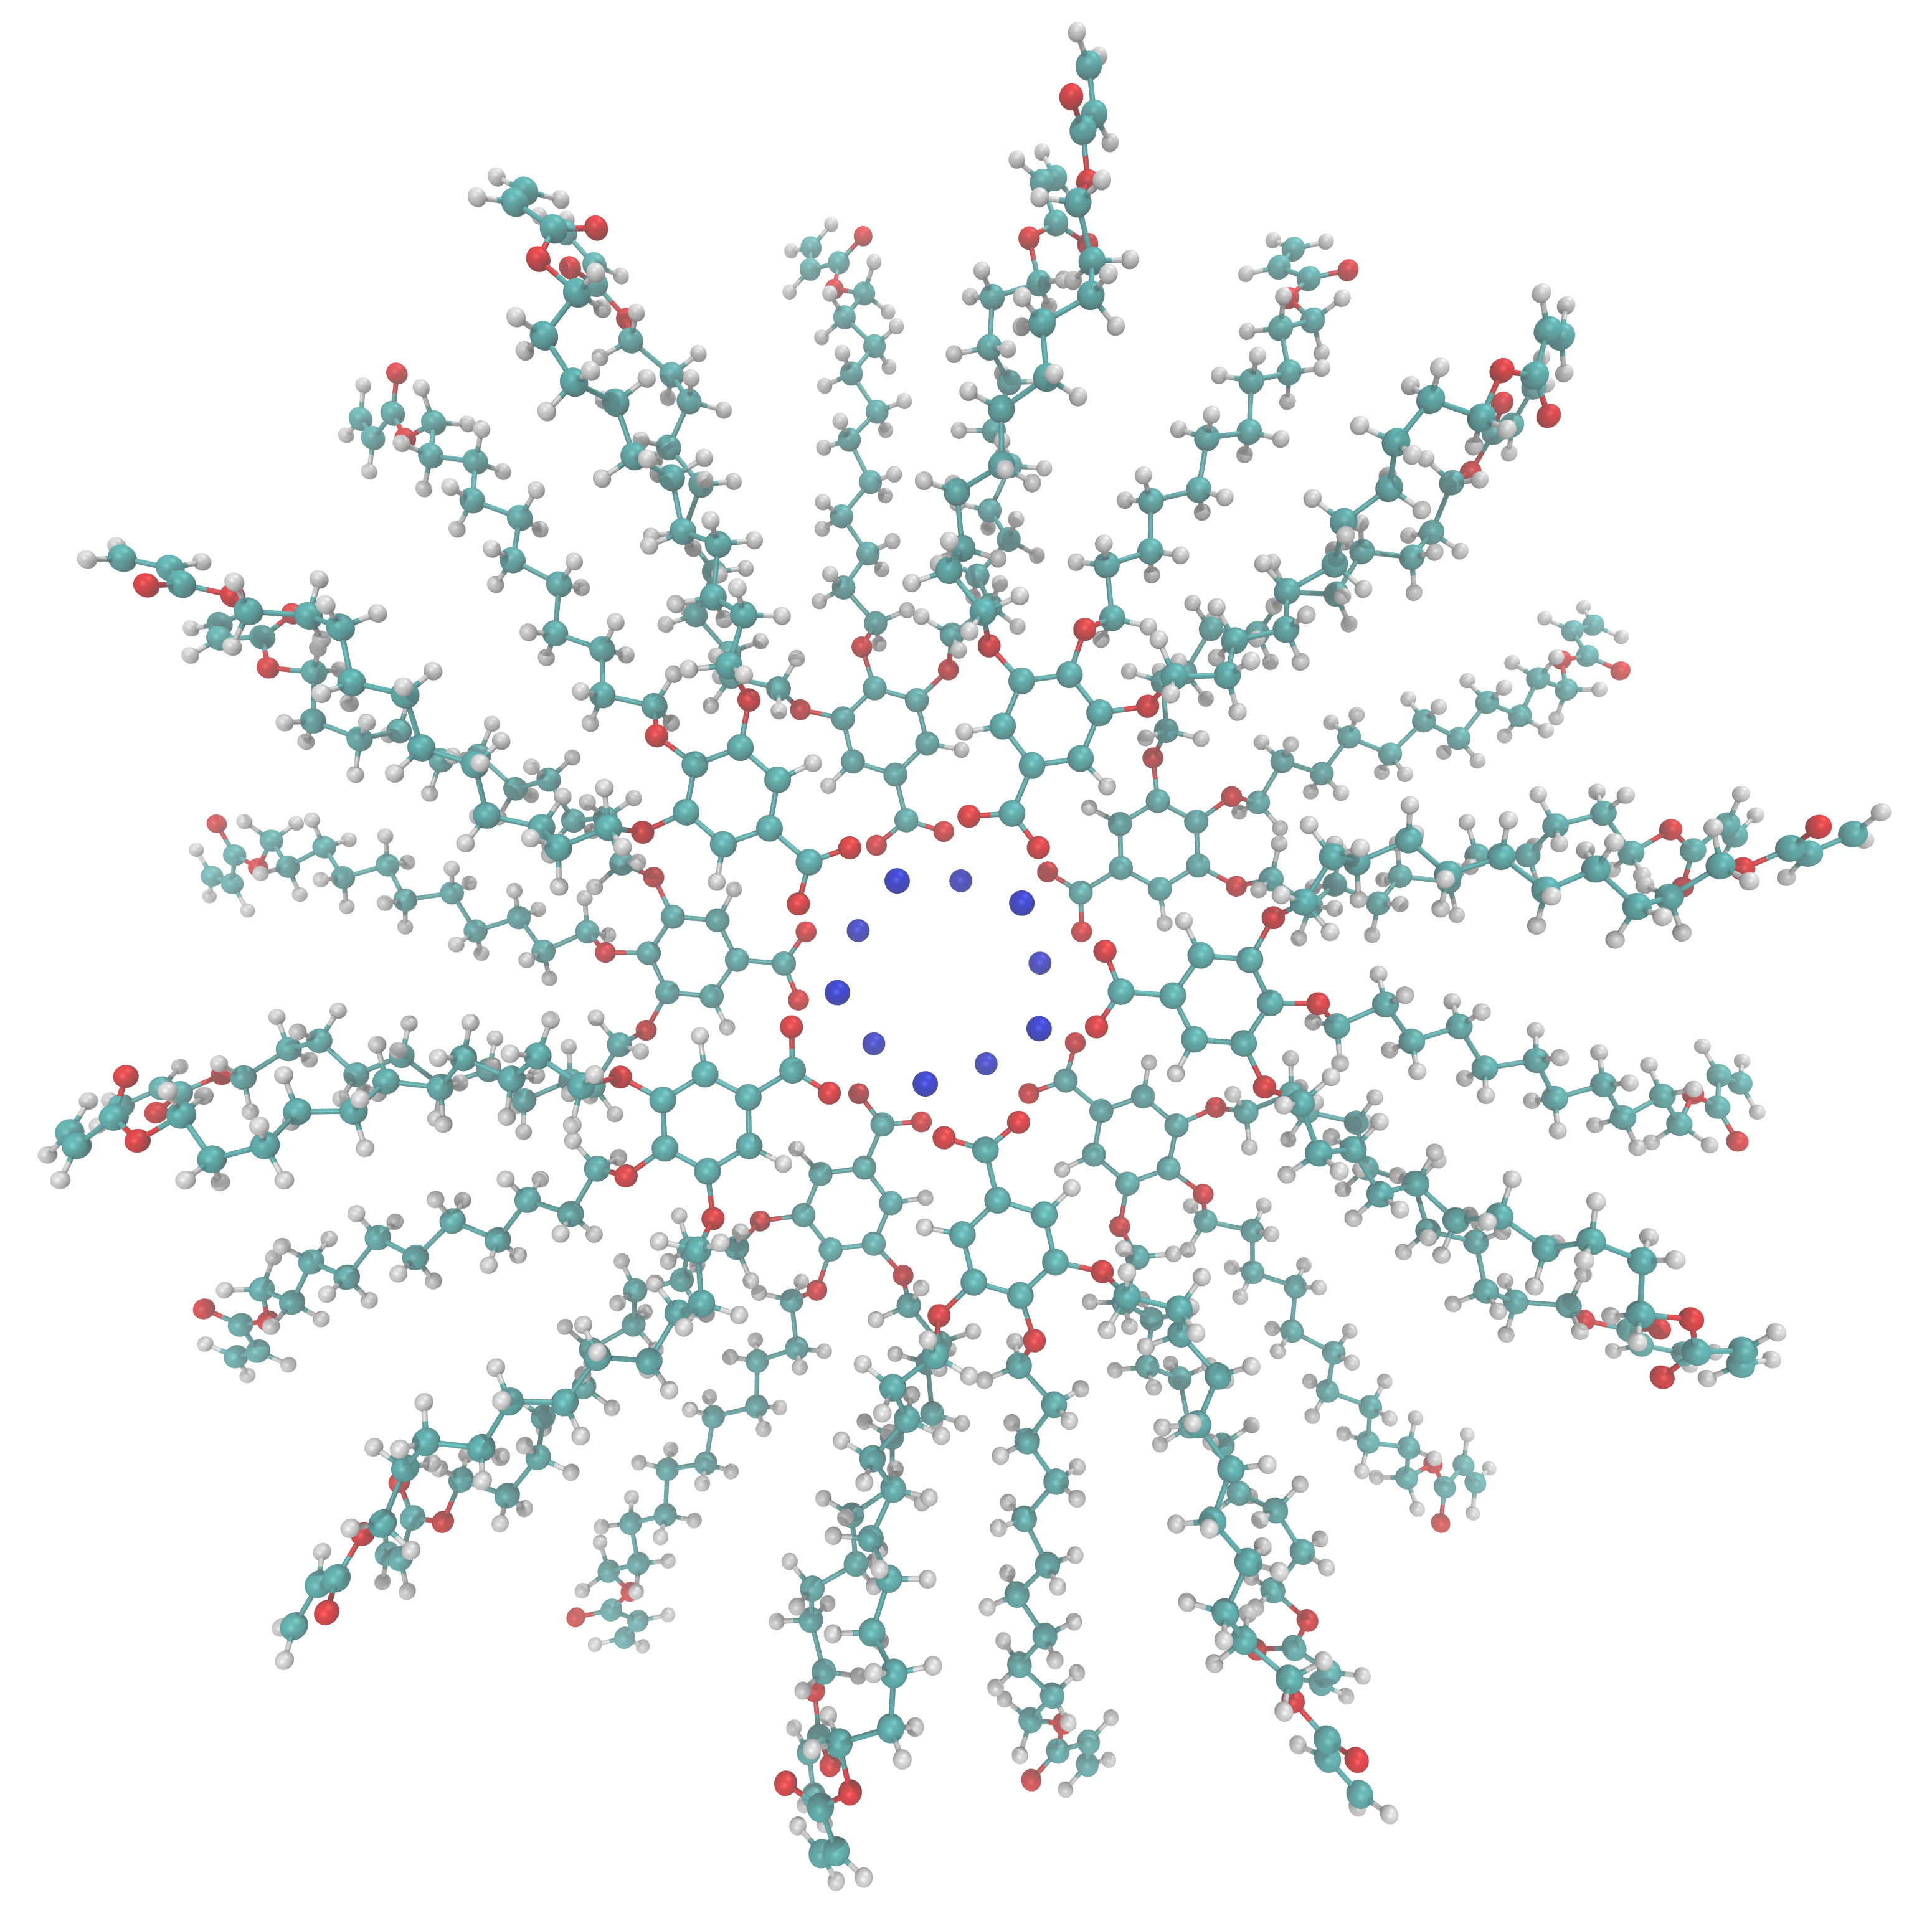
\includegraphics[width=\textwidth]{offsetlayers.png}
                \caption{}\label{fig:offsetlayers}
        \end{subfigure}
        \caption{(a) Sandwiched benzene dimers stack 3.8 \angstrom~apart. (b) Parallel-Displaced benzene dimers stack
        3.4 \angstrom~vertically and 1.6 \angstrom~horizontally apart. (c) T-shaped benzene dimers stack 5.0 \angstrom~apart.
        (d) Two monomer layers stacked in the sandwiched configuration (e) Two monomer layers stacked in the parallel-displaced
        configuration }\label{fig:stacking}
  \end{figure}

  \begin{figure}
	\centering
	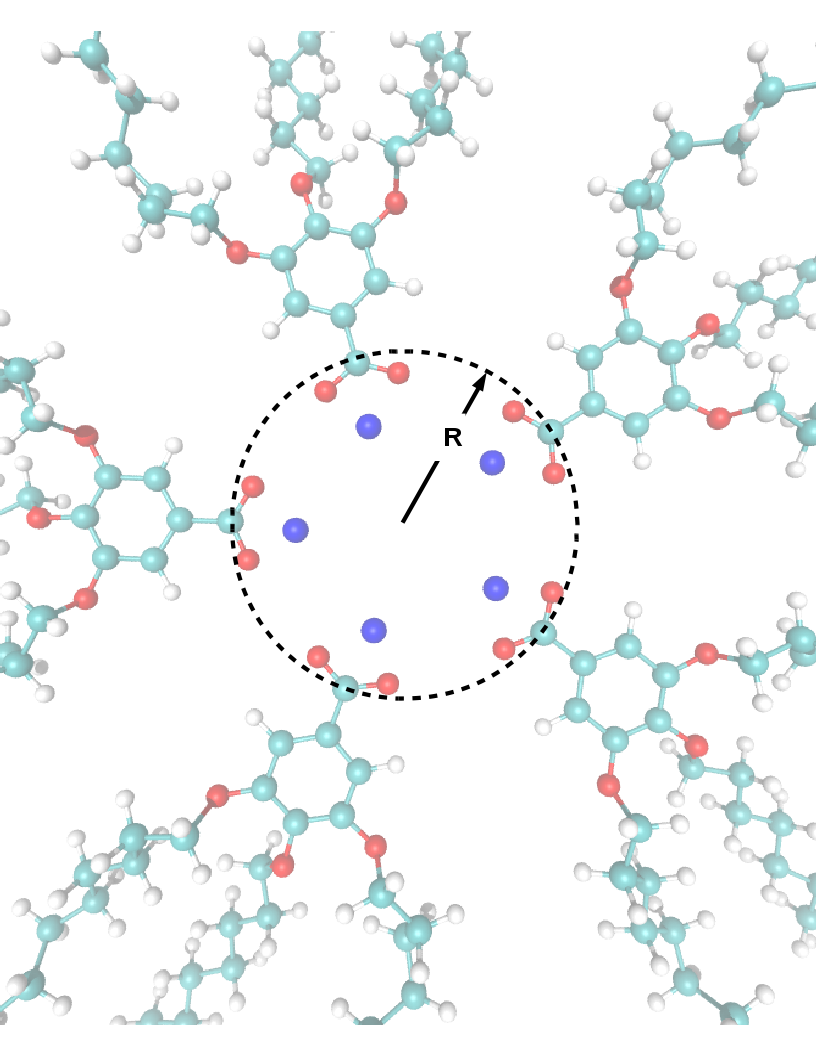
\includegraphics[width=0.8\textwidth]{pore_radius_illustration.png}
	\caption{When creating an initial configuration, the pore radius is defined based
	on the distance of the carbonyl carbon from the pore's central axis}
	\label{fig:pore_radius_illustration}
  \end{figure}

  \noindent
  \begingroup
        \fontsize{14pt}{14pt}\selectfont
	\textbf{Calculation of pore-to-pore spacing statistics}
  \endgroup
 
  \vspace{1em} 
  We are interested in 5 pore-to-pore distances which should all be
  equal in a perfect hexagonal array (Figure~\ref{fig:p2p_diagram}). Only 4 of
  the 5 distances are independent. We can calculate a trajectory of spacing
  versus time for each of the 5 distances. We calculated the average pore-to-pore
  spacing and its uncertainty according to the following procedure:
   \begin{enumerate}
	\item We calculated the time when each of the pore-to-pore distances
	were equilibrated using \\ \texttt{pymbar.timeseries.detectEquilibration()}
	\cite{chodera_simple_2016,shirts_statistically_2008}. We began calculations
	after the largest of the five values.
	\item We calculated how long it takes for the data in each of the 5
	trajectories to become uncorrelated using \texttt{pymbar.timeseries.integratedAutocorrelationTime()}
	\cite{chodera_simple_2016,shirts_statistically_2008}. 
	\item We broke the full equilibrated trajectory into blocks of length $\tau$, where
	$\tau$ is the maximum of the five autocorrelation times calculated. Each block contains
	five sub-trajectories of pore-to-pore spacings.   
	\item We generate statistics using the bootstrapping technique. For
	each bootstrap trial, we reconstruct an equilibrium trajectory by randomly
	sampling from the trajectory blocks. 
	\item The average pore-to-pore distance is the mean of all pore
	spacings among all bootstrap trials.
	\item To calculate the uncertainty in pore-to-pore distance, we calculate the average 
	pore spacing for each pore over all bootstrap trials. Using the 5 average 
	pore-to-pore distances, we calculate the spread with:
	\begin{align}
	s = \sqrt{\frac{1}{4} \sum_{i=1}^5 (x_i - \overline{x})^2} 
	\end{align}
	where $\overline{x}$ is the average pore-to-pore distance.
  \end{enumerate}

  \begin{figure}
	\centering
	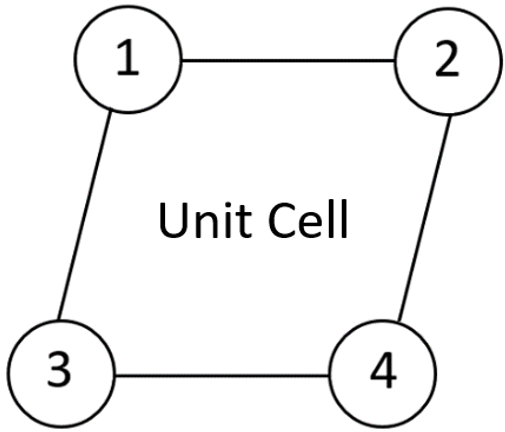
\includegraphics[width=0.25\textwidth]{p2p_diagram.png}
	\caption{There are five pore-to-pore distances that are equal in a perfect
		hexagon. If each number in the diagram represents the center of a
		pore in a hexagonal unit cell, then the distance from 1 to 2, 2 to 4, 
		4 to 3, 3 to 1 and 1 to 4 should be equal. Only 4 of the distances
		are independent. For example, the distance from 1 to 4 is defined by
		the location of all other pore centers.}
	\label{fig:p2p_diagram}
  \end{figure}

  \vspace{1em}
  \begingroup
	\fontsize{14pt}{12pt}\selectfont
	\noindent \textbf{Experimental correlation length of R-$\pi$}
  \endgroup
  
  \vspace{1em}
  Experimentalists did not measure the correlation length, so we estimated it
  from the raw data. We took a slice of the 2D WAXS data along the dashed line in
  Figure ~\ref{fig:waxs_dashed}. We removed background noise by subtracting the
  intensity far from the pattern (high $q$) uniformly. We used a least squares
  algorithm to fit a lorentzian curve to the data. Only values recorded above
  $q_z$ = 1.6 were considered for the fit in order to mitigate interference from
  R-alkanes (Figure~\ref{fig:correlation_length_exp}). The full width at half
  maximum (FWHM) is related to the correlation length, L, by the relationship: $
  L = \frac{1}{FWHM} $. The error in the value is calculated as the square root
  of the diagonal entry of the covariance matrix of optimized fit paramaters. 
  % need citations and more on lorentzian parameters
  \begin{figure}[h]
  \centering
  \begin{subfigure}{0.45\textwidth}	
  	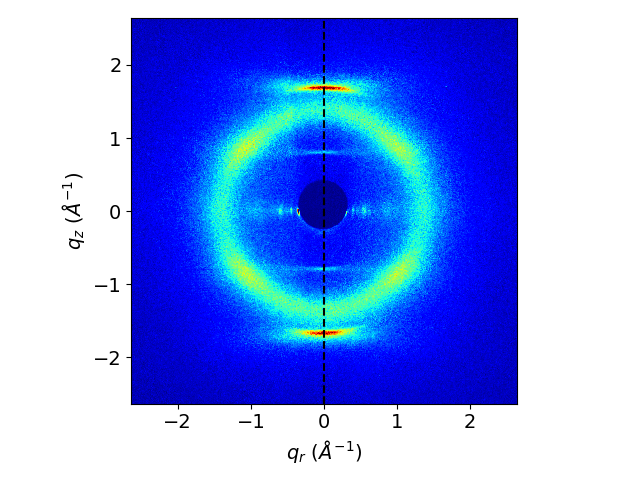
\includegraphics[width=\textwidth]{waxs_dashed.png}
	\caption{}~\label{fig:waxs_dashed}
  \end{subfigure}
  \begin{subfigure}{0.45\textwidth}
	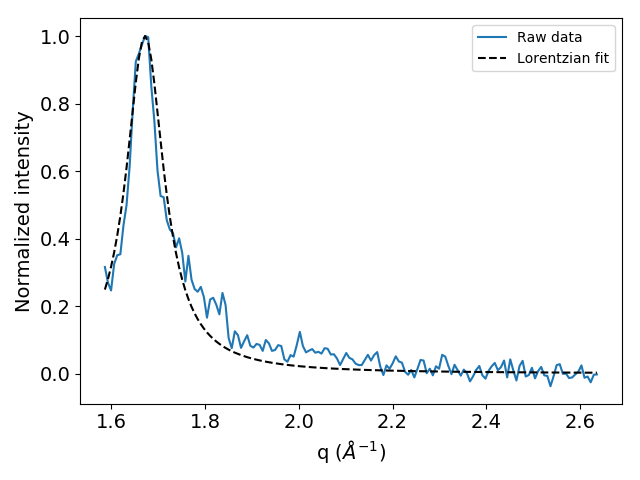
\includegraphics[width=\textwidth]{Correlation_length_exp.png}
	\caption{}~\label{fig:correlation_length_exp}
  \end{subfigure}
  \caption{}~\label{fig:correlation}
  \end{figure}
  \vspace{1em} \\
  %Our model is insensitive to initial configuration if monomer placement is chosen within reason. 
  \begingroup
	\fontsize{14pt}{12pt}\selectfont
	\textbf{Initial Configuration Dependence}
  \endgroup

  \vspace{1em}
  We addressed any major dependence on initial configuration in the main text.
  There we showed that systems are stable when made with 4, 5, 6, 7, and 8
  monomers per layer. We also showed that systems are stable when monomer head
  groups are oriented in the parallel displaced and sandwiched configurations
  (See Figure~\ref{fig:stacking}). Our model is most consistent with experiment
  when built with 5 monomers per layer, with layers stacked 3.7 \AA~apart in 
  the parallel displaced configuration. 

  There are three other parameters whose choice may influence the equilibrium
  structure: initial pore spacing, initial pore radius and initial distance
  between layers. Here we show the results of a sensitivity analysis performed
  on the three parameters. To reduce the size of the sensitivity analysis, we
  only tested systems built with 5 monomers per layer with layers stacked in 
  the parallel displaced configuration. We equilibrated all systems according
  to the dry equilibration procedure.

  \begin{enumerate}

	  \item \underline{Initial pore spacing}

	  We tested five different initial pore spacings, defined as the
	  distance between the central axis of each pore with all others
	  (Figure~\ref{fig:p2p_diagram}). To reduce the number of variables, we held the
	  pore radius constant, at 6 \AA~and the distance between layers at 3.7 \AA~since
	  those were the values used in our optimal system in the main text. We
	  prioritized ensuring that resulting configurations maintain the expected
	  hexagonal symmetry. If initial pore spacing is too small, we observe repulsion
	  between columns which disrupts equilibration. If the pore spacing is too large
	  the pores squeeze together, but in a distorted hexagonal array because the xy
	  initial translation of the pores is somewhat erratic. 

%	  If the initial pore spacing is chosen to be
%	  too small, pore columns abruptly repel each other as soon as they are able to
%	  overcome the restraining potential present as part of the dry equilibration
%	  procedure. We avoided using systems that exhibit this behavior since the
%	  behavior increases the chances of a system to become kinetically trapped in an
%	  undesired metastable free energy basin.  

	  \begin{enumerate}

		\item 39 \AA~: We tested a pore spacing of 39 \AA~in order to
		have a test system with an intial spacing below the experimental value. As soon
		as the restraining potential switches to 56 KJ mol$^{-1}$ nm$^{-2}$, the
		columns are able to repel resulting in a large jump in pore spacing
		(Figure~\ref{fig:p2p_39}). %After 400 ns, the pore spacing is 4.05 $\pm$ 0.17 nm.
%		There is a large uncertainty in this value because the 1-4 pore spacing
%		(Figure~\ref{fig:p2p_diagram}) deviates significantly from all other pore
%		spacings. The 1-4 pore spacing is 4.31 nm while the average of all other pore
%		spacings is 3.96 nm. The system deviates from hexagonal geometry and is trending
%                towards cubic packing.

		\item 41 \AA~: We chose to test a pore spacing of 41 \AA~since
		it closely matches the experimental pore spacing. Again, we observe abrupt
		repulsion of columns once the restraining potential is switched to 56 KJ
		mol$^{-1}$ nm$^{-2}$ (Figure~\ref{fig:p2p_41}). %After 400 ns, the
%		average pore spacing settles below the experimental value at 4.07 $\pm$ 0.21
%		nm. Again, a large uncertainty in this value occurs because the 1-4 pore spacing
%		(Figure~\ref{fig:p2p_diagram}) deviates significantly from all other pore
%		spacings. The 1-4 pore spacing is 4.44 nm while the average of all other pore
%		spacings is 3.96 nm. 

		\item 45 \AA~: A pore spacing of 45 \AA~is about 10 \% larger
		than the experimental value. This systems exhibits the smallest response to our 
 		equilibration procedure (Figure~\ref{fig:p2p_45}) and we chose to use this
                value for all our simulations in the main text.
f		%The equilibrated pore spacing is 4.23 $\pm$ 0.03 nm.
		%The system maintains hexagonal symmetry and exhibits the lowest uncertainty in
		%pore spacing. We chose to use this value for all our simulations in the main
		%text. 

		\item 50 \AA~: We tested a pore spacing of 50 \AA, about 20 \%
		larger than the experimental value. Once the restraining potential reaches 56
		KJ mol$^{-1}$ nm$^{-2}$, the pore spacing begins to decrease rapidly, following
		a linear trend (Figure~\ref{fig:p2p_50}).
%		After 400 ns, the average pore spacing is 4.37 $\pm$ 0.13 nm.
%		There is a large
 %               uncertainty with this value because, again, the array of pores deviates from 
 %               hexagonal character. Using Figure ~\ref{fig:p2p_diagram} as a reference, pore 
  %              2 drifts outward from the array and forces the 1-4 distance to shrink in 
   %             response.
                
		\item 55 \AA~: We tested a pore spacing of 55 \AA~which is at
		a distance where monomers in each pore no longer intersect adjacent pores. Once
		the restraining potential reaches 56 KJ mol$^{-1}$ nm$^{-2}$, the pore spacing
		changes erratically until it begins to settle when the force constants are
		below 3 KJ mol$^{-1}$ nm$^{-2}$ (Figure~\ref{fig:p2p_55}). We reccomend
		avoiding a system such as this where vacuum gaps between pore columns are
		introduced unnecessarily. %The system equilibrates to a pore spacing of 4.27
%		$\pm$ 0.18 nm. The 1-2 pore spacing is the outlier in this case with a pore
 %               spacing of 3.99 \AA~ which distorts the hexagonal array. 

	  \end{enumerate} 

	  \begin{figure}
		\centering
		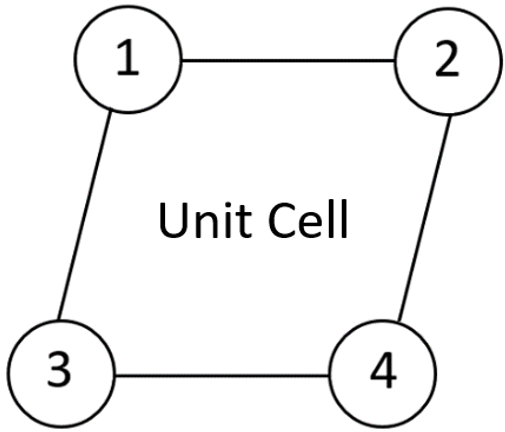
\includegraphics[width=0.4\textwidth]{p2p_diagram.png}
		\caption{In a perfect hexagonal, there are 5 distances that should be exactly
		equal. As pictured in this diagram the distance from 1-2, 1-3, 1-4, 2-4, and 3-4
		are the same.}~\label{fig:p2p_diagram}
	  \end{figure} 

	  %BJC: Could put vertical lines to indicate where position restraint values are reduced
  	  \begin{figure}[htp]
		\centering
		\begin{subfigure}{0.3\textwidth}
			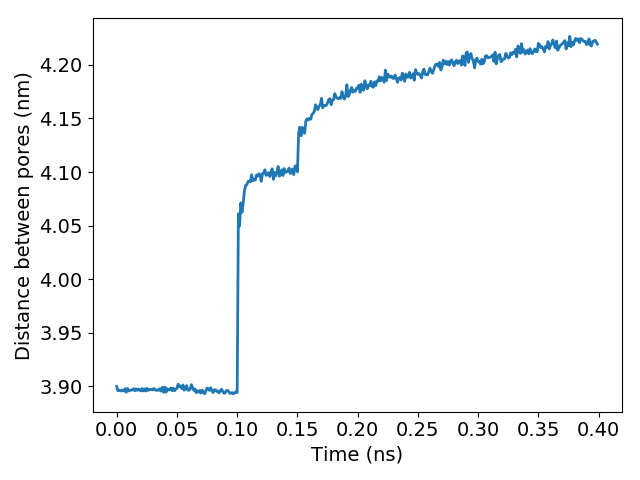
\includegraphics[width=\textwidth]{p2p_39.png}\quad
			\vspace{-1.25em}
			\caption{39 \AA~initial pore spacing}~\label{fig:p2p_39}
		\end{subfigure}
		\begin{subfigure}{0.3\textwidth}
			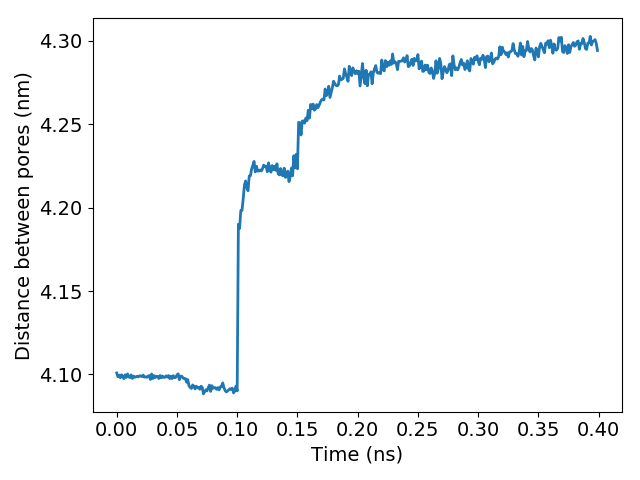
\includegraphics[width=\textwidth]{p2p_41.png}\quad
			\vspace{-1.25em}
			\caption{41 \AA~initial pore spacing}~\label{fig:p2p_41}
		\end{subfigure}
		\begin{subfigure}{0.3\textwidth}
			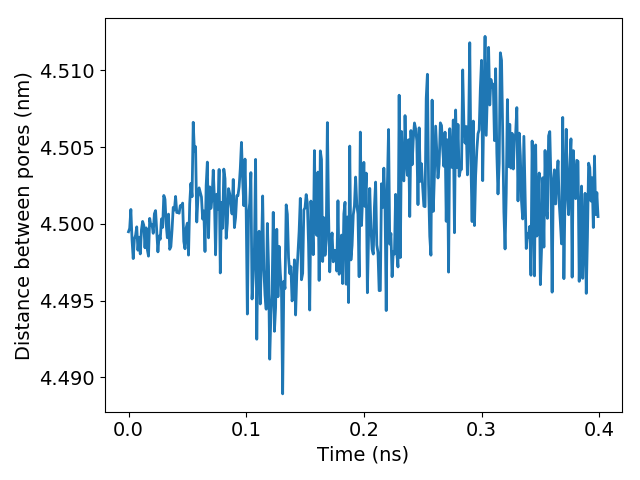
\includegraphics[width=\textwidth]{p2p_45.png}
			\vspace{-1.25em}
			\caption{45 \AA~initial pore spacing}~\label{fig:p2p_45}
		\end{subfigure}
		\begin{subfigure}{0.3\textwidth}
			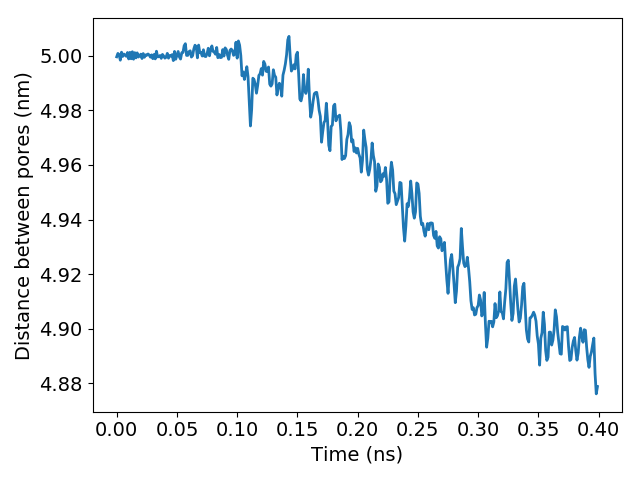
\includegraphics[width=\textwidth]{p2p_50.png}\quad	
			\vspace{-1.25em}
			\caption{50 \AA~initial pore spacing}~\label{fig:p2p_50}
		\end{subfigure}
		\begin{subfigure}{0.3\textwidth}
			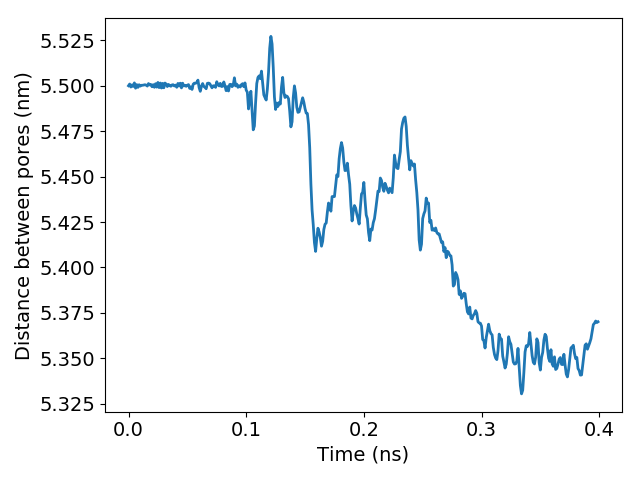
\includegraphics[width=\textwidth]{p2p_55.png}
			\vspace{-1.25em}
			\caption{55 \AA~initial pore spacing}~\label{fig:p2p_55}
		\end{subfigure}

		\caption{The pore spacing during the restrained portion of the
			dry equilibration procedure is shown. Every 50 ps (0.05 ns) position restraints
			are reduced according to the sequence: 1000000, 3162, 56, 8, 3, 2, 1, 0 KJ
			mol$^{-1}$ nm$^{-2}$. When the initial pore spacing is chosen below the
			experimental value (a) or at the experimental value (b), there is an abrupt
			change in pore spacing when the position restraints are reduced to 56 KJ
			mol$^{-1}$ nm$^{-2}$. When pores are started 45 \AA~apart (c) the pore spacing
			remains relatively stable. When pores are spaced 50 \AA~apart (d), the pore
			spacing decreases nearly linearly once the restraints are reduced to 56 KJ
			mol$^{-1}$ nm$^{-2}$. When pores are spaced 55 \AA~apart (e), so that monomers
			do not intersect with adjacent pores, and position restraints are reduced to 56
			KJ mol$^{-1}$ nm$^{-2}$, the pore spacing changes erratically before stabilizing
			when force constants are reduced below 3 KJ mol$^{-1}$ nm$^{-2}$.} 
		\label{fig:p2p}
	  \end{figure}

	  \item \underline{Initial pore radius}

	  We tested 3 different pore radii, defined as shown in
	  Figure~\ref{fig:pore_radius_illustration}. For each system, we held the initial
	  pore spacing constant at 45 \AA~and the initial distance between layers
	  constant at 3.7 \AA. Equilibrated values of pore radii are presented in
	  Table~\ref{table:radii}. The pore radius in each simulation frame is calculated
	  as the average distance of all carbonyl carbons (See
	  Figure~\ref{fig:pore_radius_illustration}) from their associated pore center.
	  Statistics for the pore radii reported were generated from the timeseries
	  representing the average pore radius at each frame. We detected equilibration
	  using \texttt{pymbar.timeseries.detectEquilibration}. We calculated the average
	  and standard deviation of pore radii using only data points collected after
	  equilibration was detected.

	  \begin{enumerate}

		\item 2.5 \AA~: The smallest pore radius that we can achieve
		before energy minimization becomes problematic is 2.5 \AA. After being run
		through the full dry equilibration procedure, the average pore radius is 0.40
		$\pm$ 0.01 \AA.

		\item 5 \AA~: We tested a pore radius of 5 \AA~because it is
		slightly larger than the equilibrated pore radius of the system simulated with
		an intial pore radius of 2.5 \AA. After being run through the full dry
		equilibration procedure, the average pore radius is 0.42 $\pm$ 0.01 \AA, which
		agrees with the 2.5 \AA~configuration within error. 

		\item 8 \AA~: The largest pore radius that can achieved before
		energy minimization becomes problematic is 8 \AA. One should use caution with
		such a structure because of the relatively large vacuum space that is created
		in the pore region of the initial configuration. After being run through the
		full dry equilibration procedure, we see a combination of cylindrical and
		slit-like pores (Figure~\ref{fig:slits}). Measuring the pore radius of this
		system does not have a concrete meaning since slits do not have a single
		radius, but its calculated value is reported in Table ~\ref{table:radii}. We
		are wary of such a non-symmetric structure and choose not to use a pore radius
		of 8 \AA~for our starting configurations. 
	  
	  \end{enumerate}

	  \begin{table}[h]
	  \centering
	  \begin{tabular}{cc}
	  \toprule
	  Initial Pore Radius & Equilibrated Pore Radius \\
	  \midrule
	  % BJC: to be updated once simulations are run out long enough
	  2.5 \AA & $0.40 \pm 0.01$ \AA \\
	  5 \AA   & $0.42 \pm 0.01$ \AA \\ % final result
	  8 \AA   & $0.69 \pm 0.01$ \AA \\
	  \bottomrule
	  \end{tabular}
	  \caption{The average pore radii of systems built with an initial pore
		  radius of 2.5 \AA~and 5 \AA~equilibrate to values that agree within error. If
		  the pore radius is too large, slit pores may form.}~\label{table:radii}
	  \end{table}

	  \begin{figure}
	  \centering
          \includegraphics[width=\textwidth]{slit_pores.png}
	  \caption{A system that was built with an initial pore radius of 8
		  \AA~equilibrates to a structure that exhibits both cylindrical and slit-like
		  pores. As pictured here, sodium ions are colored blue, carbon atoms in the
		  aromatic ring of the head group are colored orange and all else is colored
		  cyan.}~\label{fig:slits}
	  \end{figure}

	  \item \underline{Initial distance between layers}

	  We tested 3 different initial layer spacings, defined as the distance
	  between the planes of aromatic rings in each layer. Systems built with layers
	  stacked 3.7 \AA~and 5 \AA~apart are discussed extensively in the main text. We
	  will focus the discussion here on systems built with layers stacked 10 \AA~
	  apart.

	  Figure~\ref{fig:dbwl_10} shows the structure of an assembly built
	  with an initial layer spacing of 10 \AA~immediately after the restrained
	  portion of the equilibration procedure. Since we used position restraints, the
	  simulations were run in the NVT ensemble. When layer spacing is large, such as
	  this situation, there is a significant amount of vacuum space which the monomer
	  attempts to fill. Even if turning pressure control on allows the system to
	  recover the geometry of the hexagonal phase, we would likely need much longer
	  equilibration times, and it will almost certainly get trapped in a metastable
	  configuration that bears no resemblence to the experimental profile. 
 
	  \begin{figure}
		\centering
		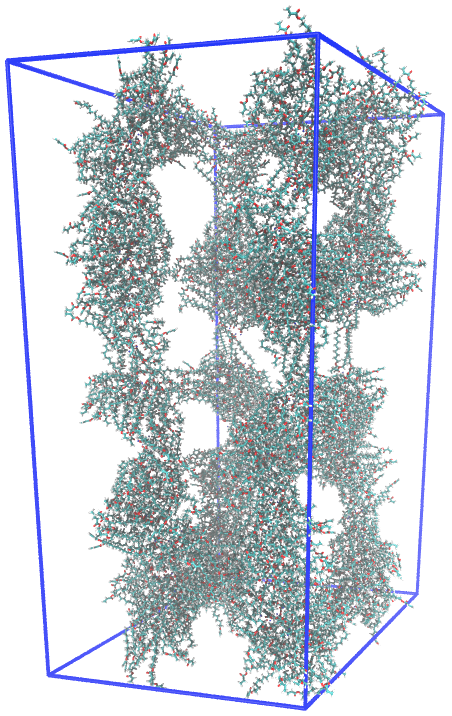
\includegraphics[width=0.5\textwidth]{dbwl_10.png}
		\caption{When layers are initially stacked 10 \AA~apart and the system
                is equilibrated using the dry equlibration procedure, large vacuum gaps
		form as the monomers attempt to fill space.}\label{fig:dbwl_10} 
	  \end{figure}

  \end{enumerate}

  \begin{figure}
	\centering
        \begin{subfigure}{0.40\textwidth}
                \centering
                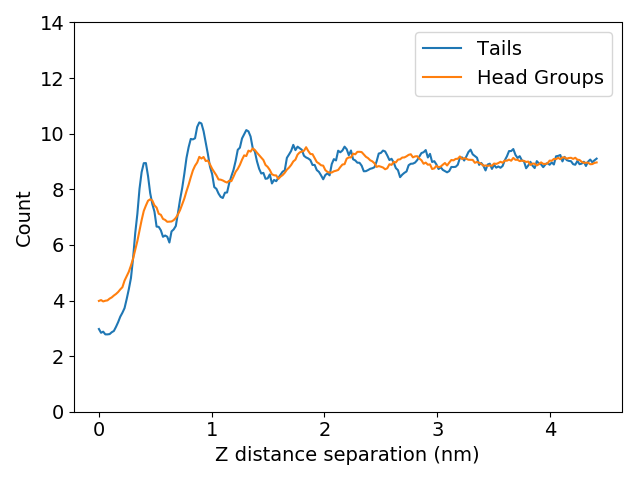
\includegraphics[width=\textwidth]{zdf_layered_4.png}
                \caption{4 mon/layer, Sandwiched}\label{fig:zdf_layered_4}
        \end{subfigure}
        \begin{subfigure}{0.40\textwidth}
                \centering
                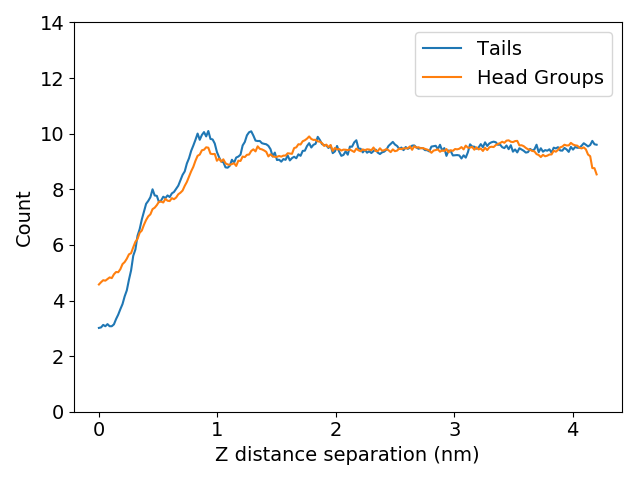
\includegraphics[width=\textwidth]{zdf_offset_4.png}
                \caption{4 mon/layer, Parallel Displaced}\label{fig:zdf_layered_4}
        \end{subfigure}
	\begin{subfigure}{0.40\textwidth}
                \centering
                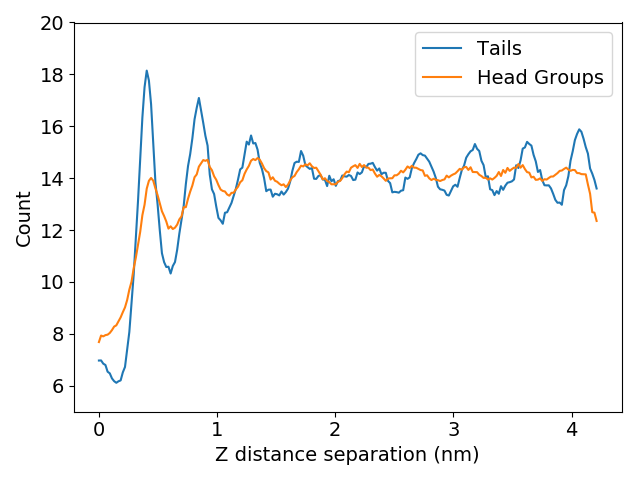
\includegraphics[width=\textwidth]{zdf_layered_6.png}
                \caption{6 mon/layer, Sandwiched}\label{fig:zdf_layered_6}
        \end{subfigure}
        \begin{subfigure}{0.40\textwidth}
                \centering
                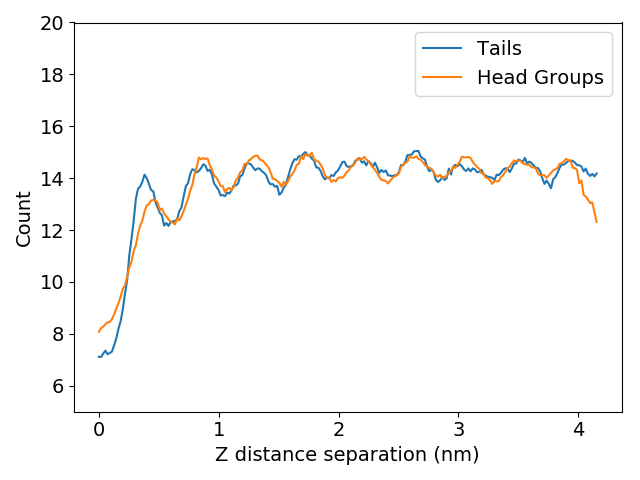
\includegraphics[width=\textwidth]{zdf_offset_6.png}
                \caption{6 mon/layer, Parallel Displaced}\label{fig:zdf_layered_6}
        \end{subfigure}
        \begin{subfigure}{0.40\textwidth}
                \centering
                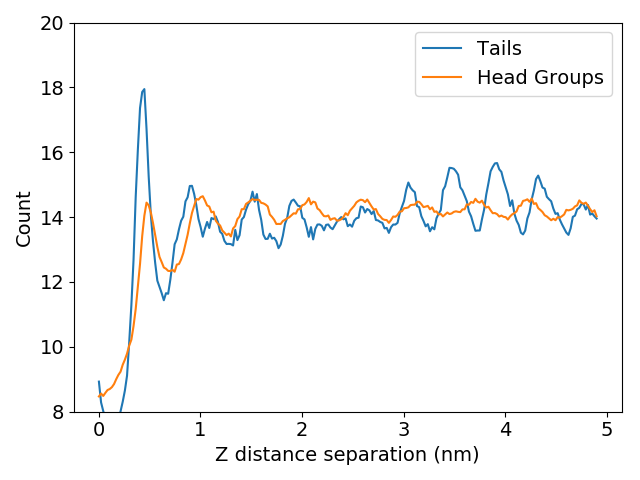
\includegraphics[width=\textwidth]{zdf_layered_7.png}
                \caption{7 mon/layer, Sandwiched}\label{fig:zdf_layered_7}
        \end{subfigure}
        \begin{subfigure}{0.40\textwidth}
                \centering
                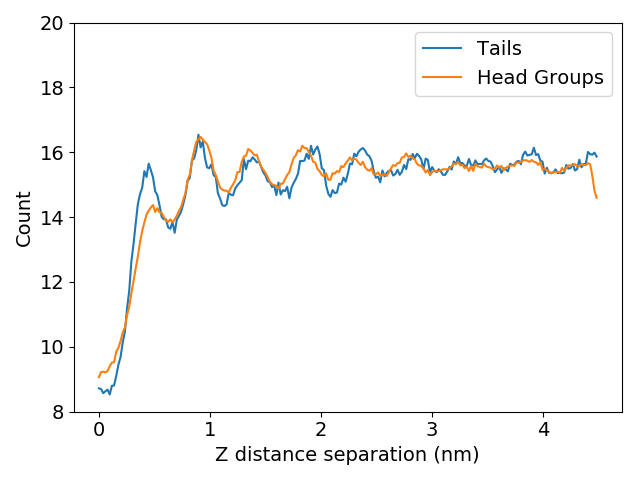
\includegraphics[width=\textwidth]{zdf_offset_7.png}
                \caption{7 mon/layer, Parallel Displaced}\label{fig:zdf_layered_7}
        \end{subfigure}
	\begin{subfigure}{0.40\textwidth}
                \centering
                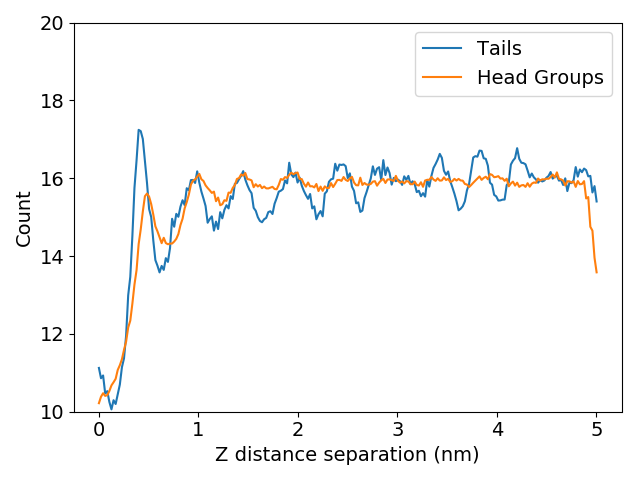
\includegraphics[width=\textwidth]{zdf_layered_8.png}
                \caption{8 mon/layer, Sandwiched}\label{fig:zdf_layered_8}
        \end{subfigure}
        \begin{subfigure}{0.40\textwidth}
                \centering
                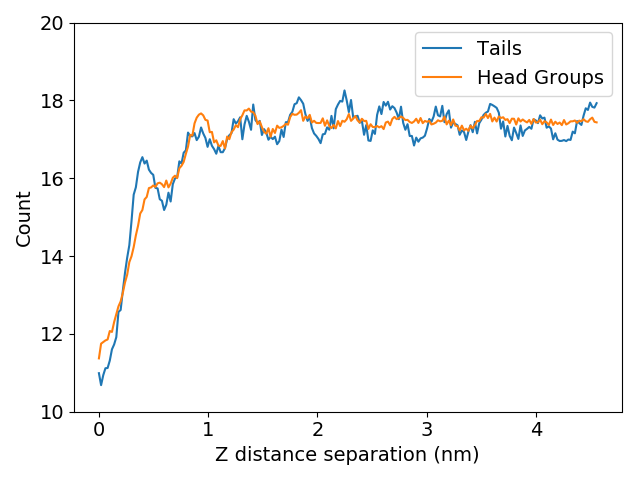
\includegraphics[width=\textwidth]{zdf_offset_8.png}
                \caption{8 mon/layer, Parallel Displaced}\label{fig:zdf_layered_8}
        \end{subfigure}
	\caption{$g(z)$ for all other configurations built with layers stacked 3.7 \AA~apart}\label{fig:zdf}
  \end{figure}

  \begin{figure}
	\centering
        \begin{subfigure}{0.40\textwidth}
                \centering
                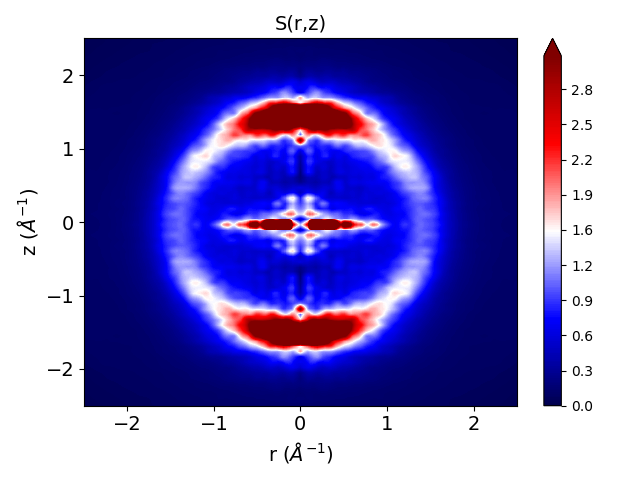
\includegraphics[width=\textwidth]{rzplot_layered_4.png}
                \caption{4 mon/layer, Sandwiched}\label{fig:rzplot_layered_4}
        \end{subfigure}
        \begin{subfigure}{0.40\textwidth}
                \centering
                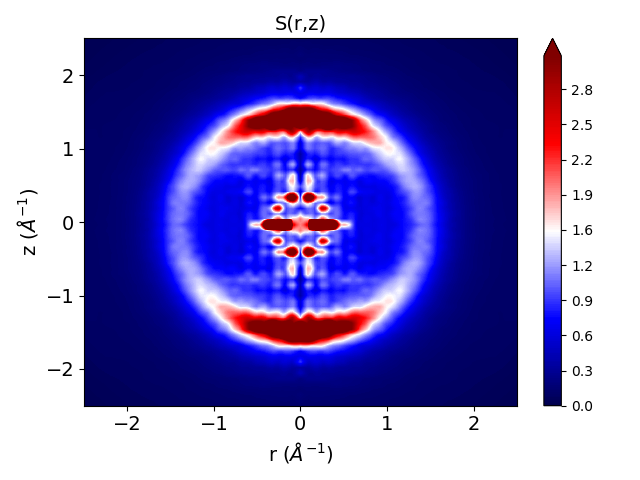
\includegraphics[width=\textwidth]{rzplot_offset_4.png}
                \caption{4 mon/layer, Parallel Displaced}\label{fig:rzplot_offset_4}
        \end{subfigure}
        \begin{subfigure}{0.40\textwidth}
                \centering
                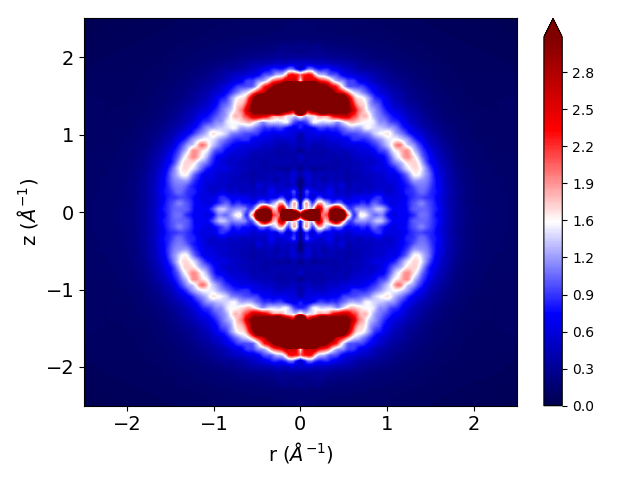
\includegraphics[width=\textwidth]{rzplot_layered_6.png}
                \caption{6 mon/layer, Sandwiched}\label{fig:rzplot_layered_6}
        \end{subfigure}
        \begin{subfigure}{0.40\textwidth}
                \centering
                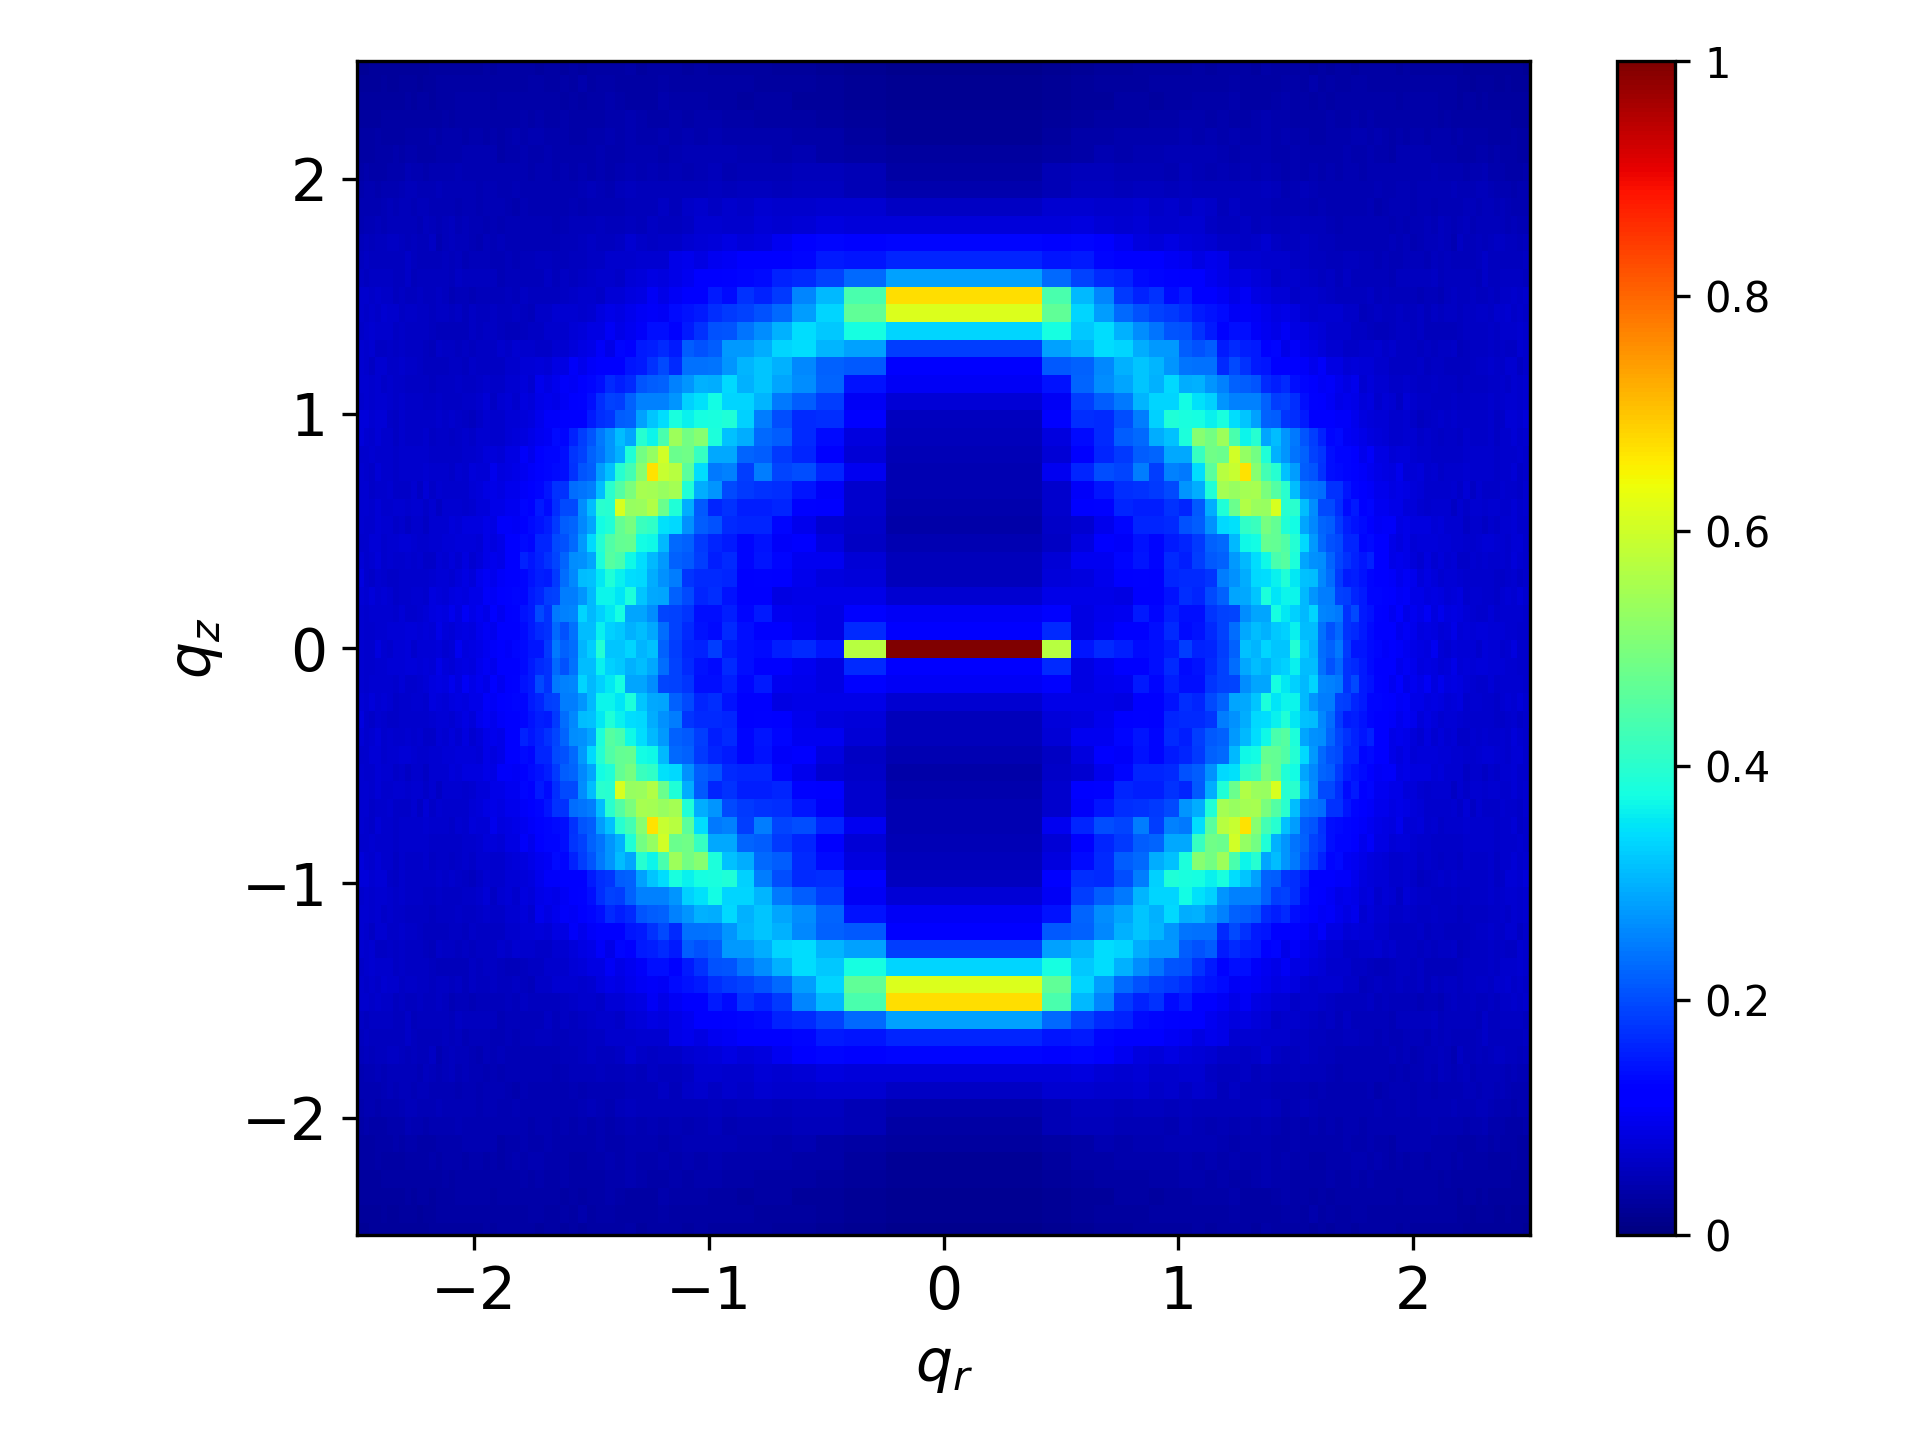
\includegraphics[width=\textwidth]{rzplot_offset_6.png}
                \caption{6 mon/layer, Parallel Displaced}\label{fig:rzplot_offset_6}
        \end{subfigure}
        \begin{subfigure}{0.40\textwidth}
                \centering
                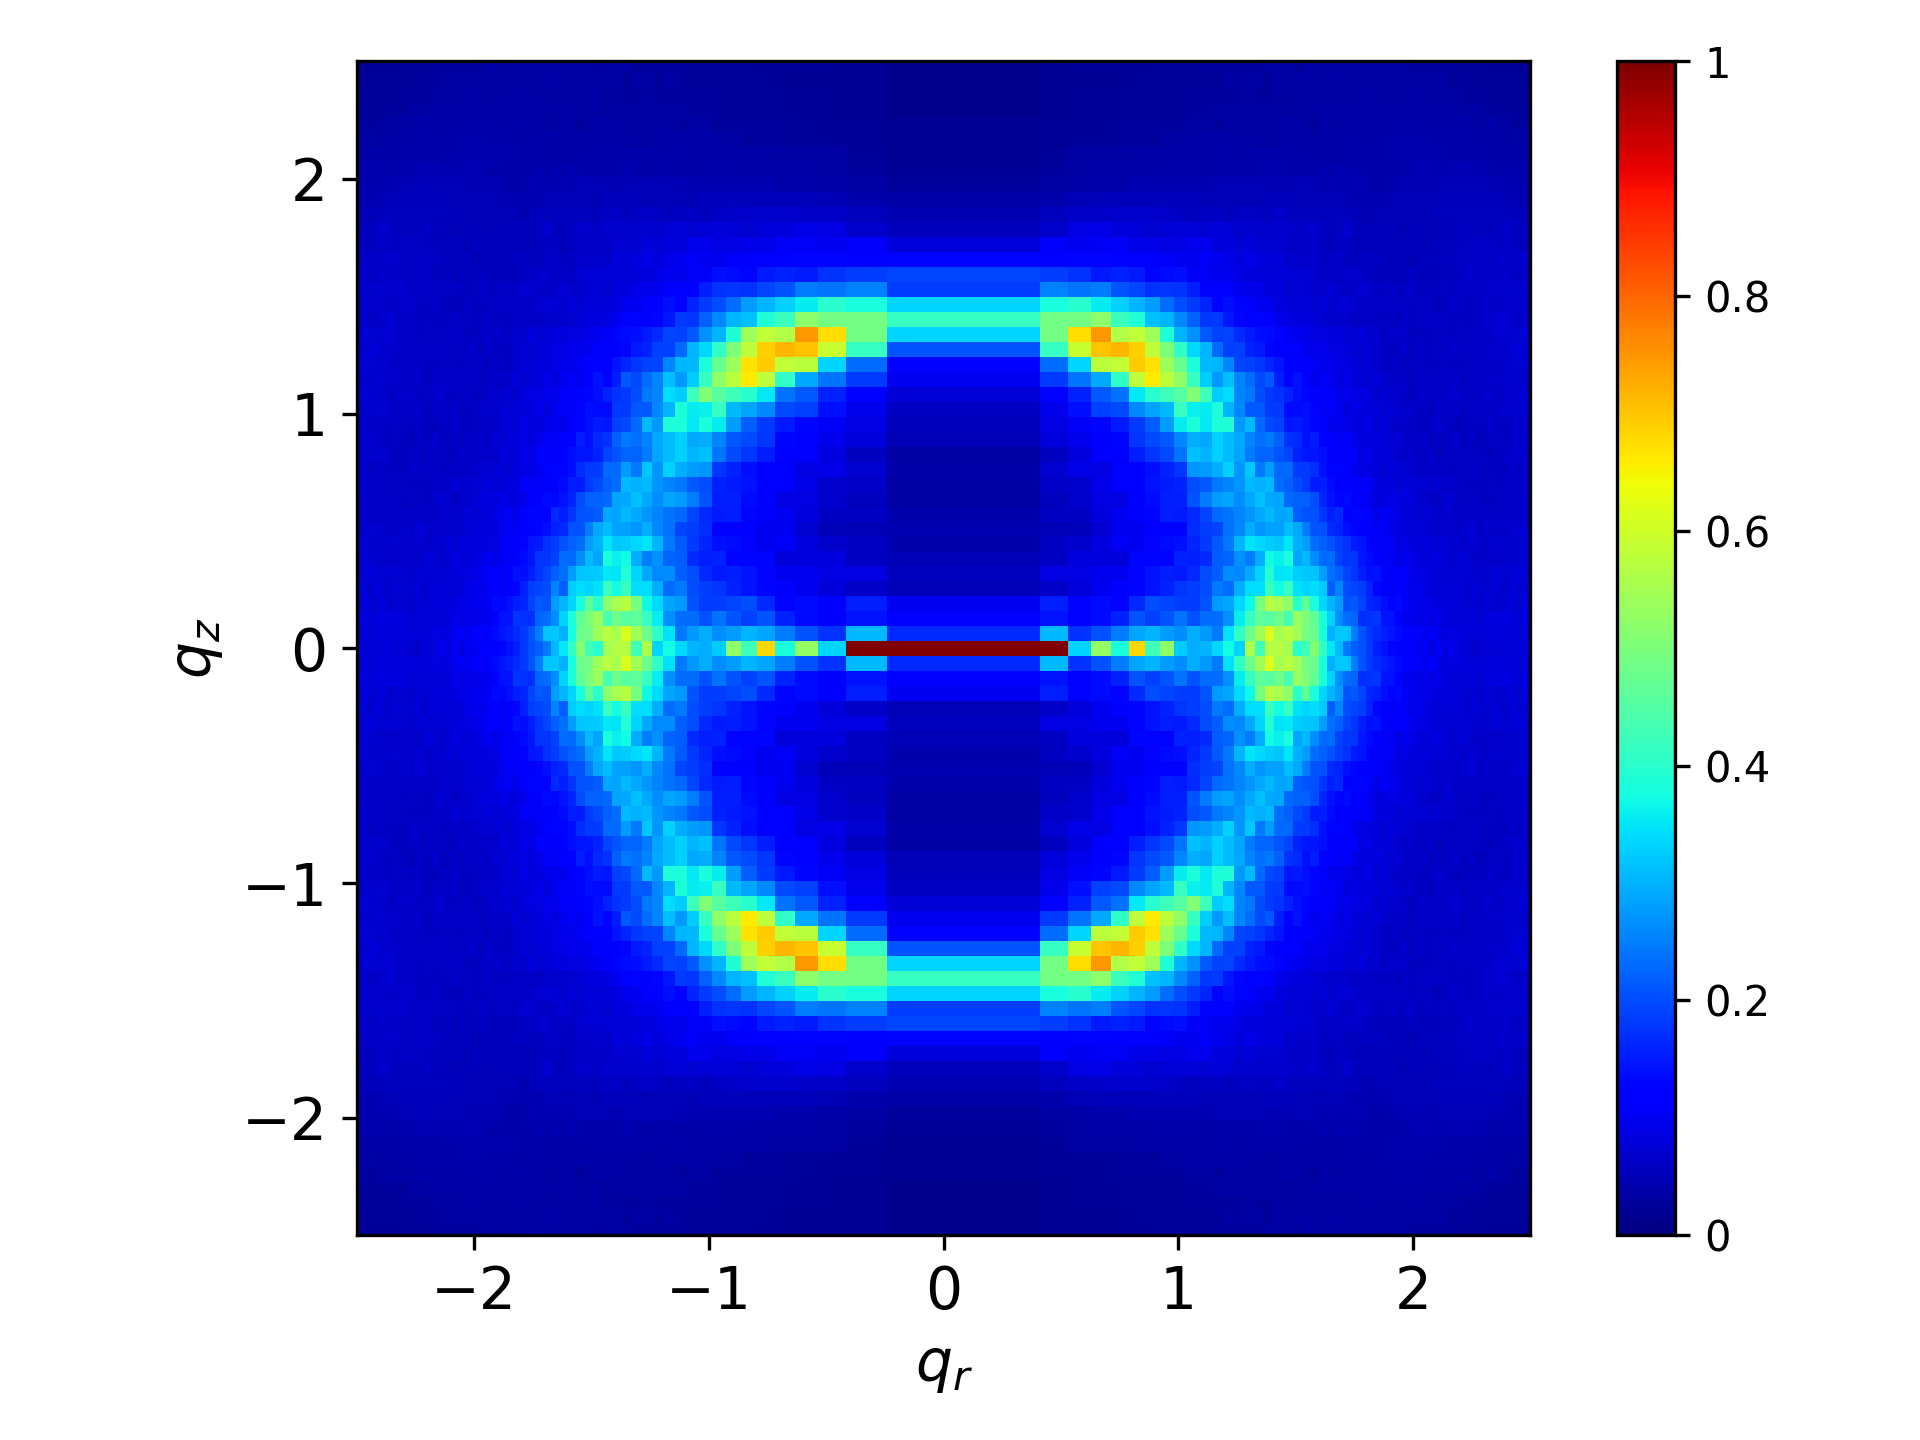
\includegraphics[width=\textwidth]{rzplot_layered_7.png}
                \caption{7 mon/layer, Sandwiched}\label{fig:rzplot_layered_7}
        \end{subfigure}
        \begin{subfigure}{0.40\textwidth}
                \centering
                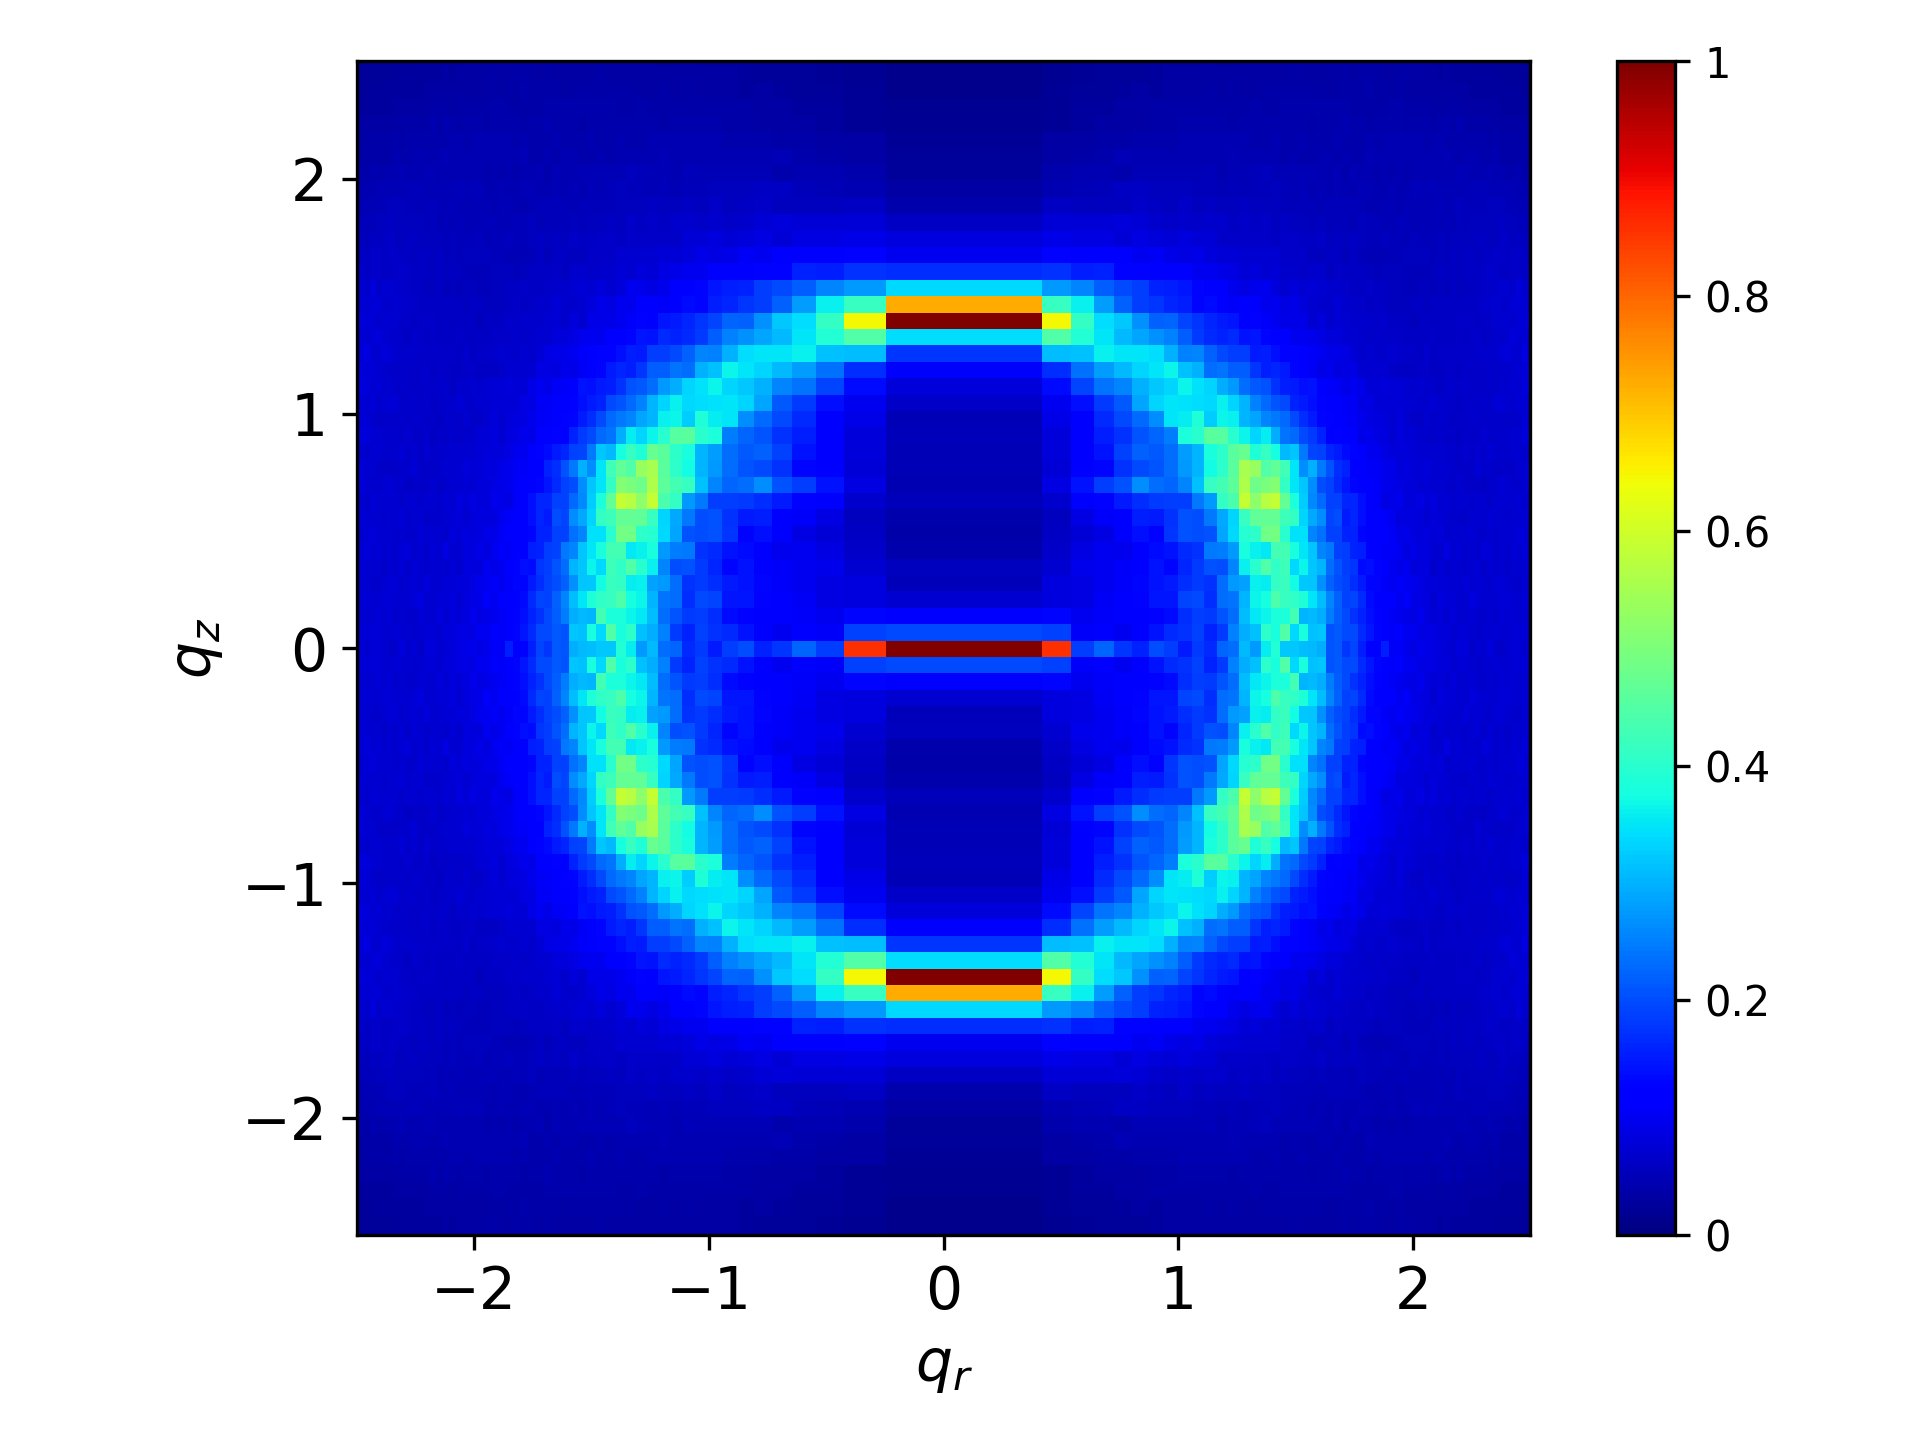
\includegraphics[width=\textwidth]{rzplot_offset_7.png}
                \caption{7 mon/layer, Parallel Displaced}\label{fig:rzplot_offset_7}
        \end{subfigure}
        \begin{subfigure}{0.40\textwidth}
                \centering
                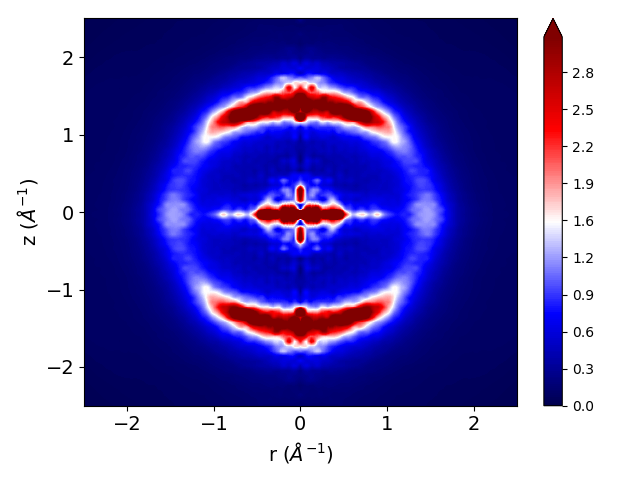
\includegraphics[width=\textwidth]{rzplot_layered_8.png}
                \caption{8 mon/layer, Sandwiched}\label{fig:rzplot_layered_8}
        \end{subfigure}
        \begin{subfigure}{0.40\textwidth}
                \centering
                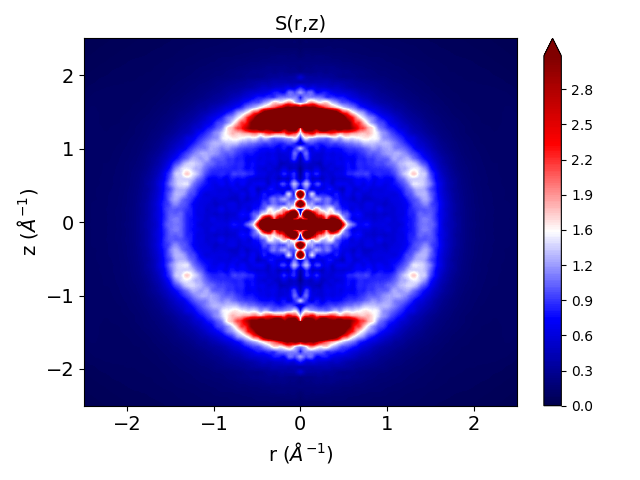
\includegraphics[width=\textwidth]{rzplot_offset_8.png}
                \caption{8 mon/layer, Parallel Displaced}\label{fig:rzplot_offset_8}
        \end{subfigure}
	\caption{Simulated XRD patterns for all other configurations built with
		 layers stacked 3.7 \AA~apart}\label{fig:XRDsim}
  \end{figure}

%  \begin{wrapfigure}{R}{0.4\textwidth}
%      \centering
%      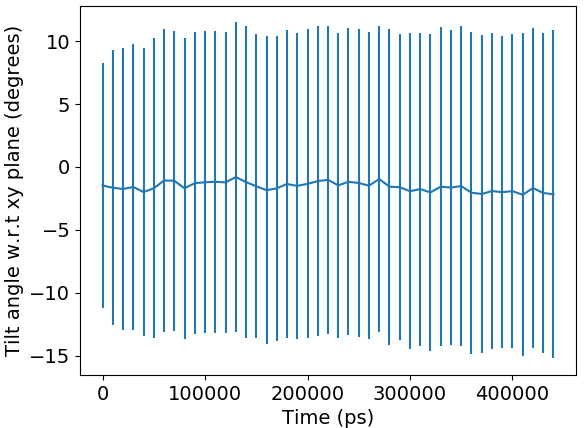
\includegraphics[width=0.4\textwidth]{tilt.png}
%      \caption{The average angle between alkane chains and the xy plane is nearly zero degrees}\label{fig:tilt}     
%  \end{wrapfigure}


%  \begin{figure}
%	\centering
%	\begin{subfigure}{0.45\textwidth}
%		\centering
%		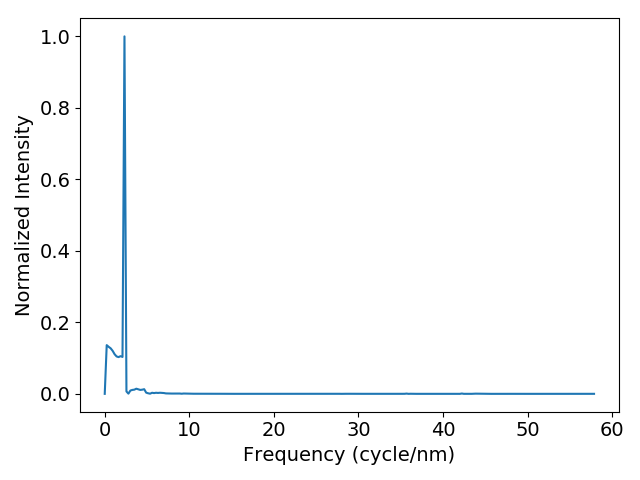
\includegraphics[width=\textwidth]{ps5layered.png}
%		\caption{}\label(fig:ps5layered}
%	\end{subfigure}
%	\begin{subfigure}
%		\centering
%		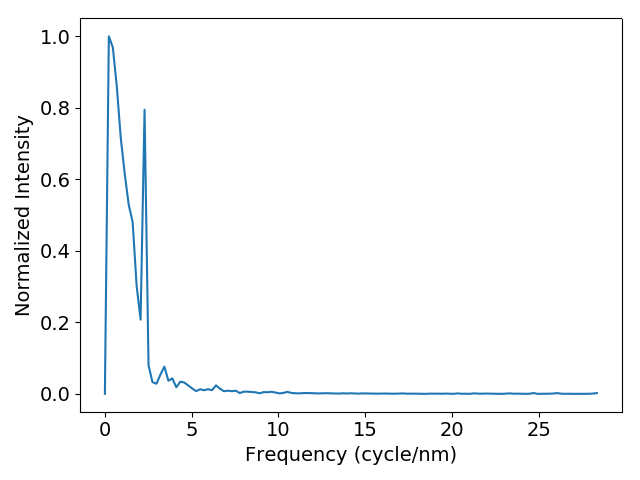
\includegraphics[width=\textwidth]{ps5offset.png}
%		\caption{}\label{fig:ps5offset}
%	\end{subfigure}
%  \end{figure}

  \begin{figure}
	\centering
	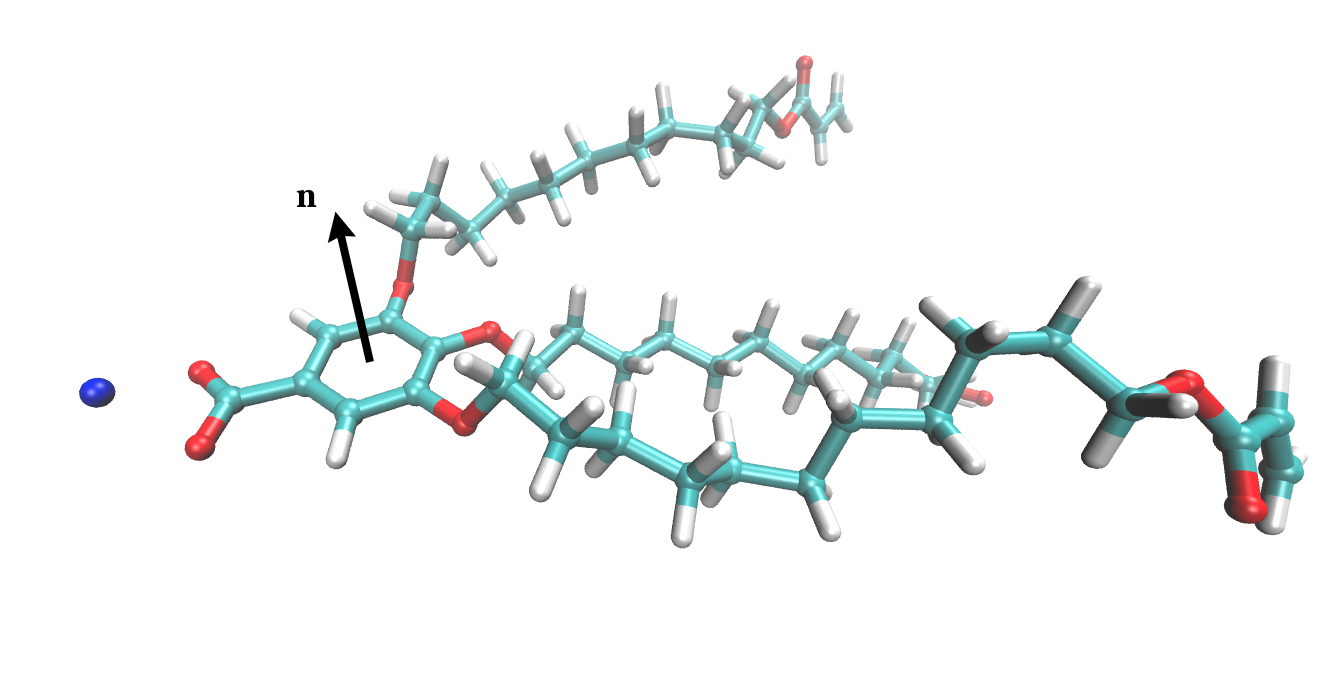
\includegraphics[width=0.75\linewidth]{nematic_director.png}
	\caption{We define the nematic director vector, $\mathbf{n}$, as the vector
	perpendicular to the plane of the aromatic head group.}~\label{fig:director}
  \end{figure}

  \begin{figure}[ht]

  \begin{subfigure}{\linewidth}
        \centering
        \begin{subfigure}{0.45\linewidth}
                \centering
                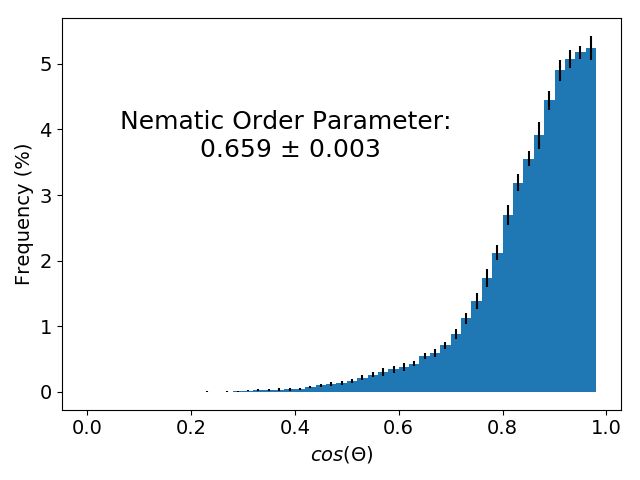
\includegraphics[width=\linewidth]{layered_nematic_order.png}
                \caption{Sandwiched, Ordered}~\label{fig:sandwich_nematic}
        \end{subfigure}%
        \begin{subfigure}{0.45\linewidth}
                \centering
                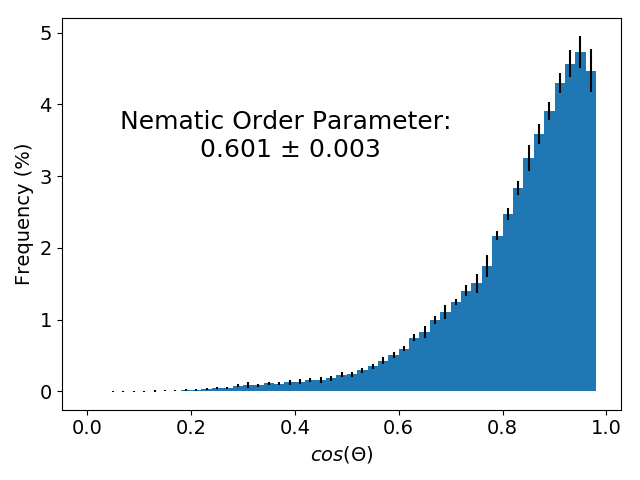
\includegraphics[width=\linewidth]{offset_nematic_order.png}
                \caption{Parallel Displaced, Ordered}~\label{fig:offset_nematic}
        \end{subfigure}
        \begin{subfigure}{0.45\linewidth}
                \centering
                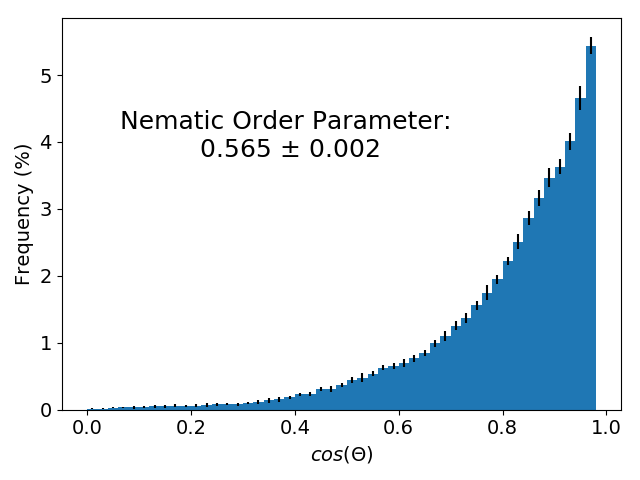
\includegraphics[width=\linewidth]{disorder_sandwich_nematic_order.png}
                \caption{Sandwiched, Disordered}~\label{fig:disorder_sandwich_nematic}
        \end{subfigure}%
        \begin{subfigure}{0.45\linewidth}
                \centering
                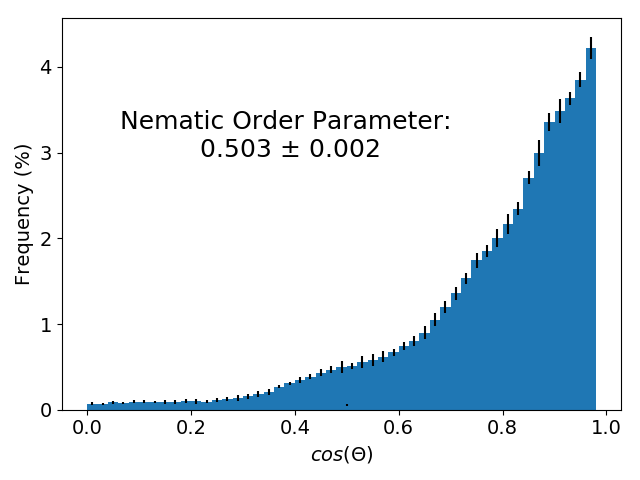
\includegraphics[width=\linewidth]{disorder_offset_nematic_order.png}
                \caption{Parallel Displaced, Disordered}~\label{fig:disorder_offset_nematic}
        \end{subfigure}

  \end{subfigure}
  \caption{The distribution of angles between nematic director vector (See
	  Figure~\ref{fig:director}) and the z-axis averaged over the equilibrated portion
	  of each trajectory}~\label{fig:nematic_distribution}
  \end{figure}

  \begin{figure}[!ht]
        \centering
%        \begin{subfigure}{0.45\textwidth}
%                \centering
%                \hspace{-1cm}
%                \vspace{1cm}
%                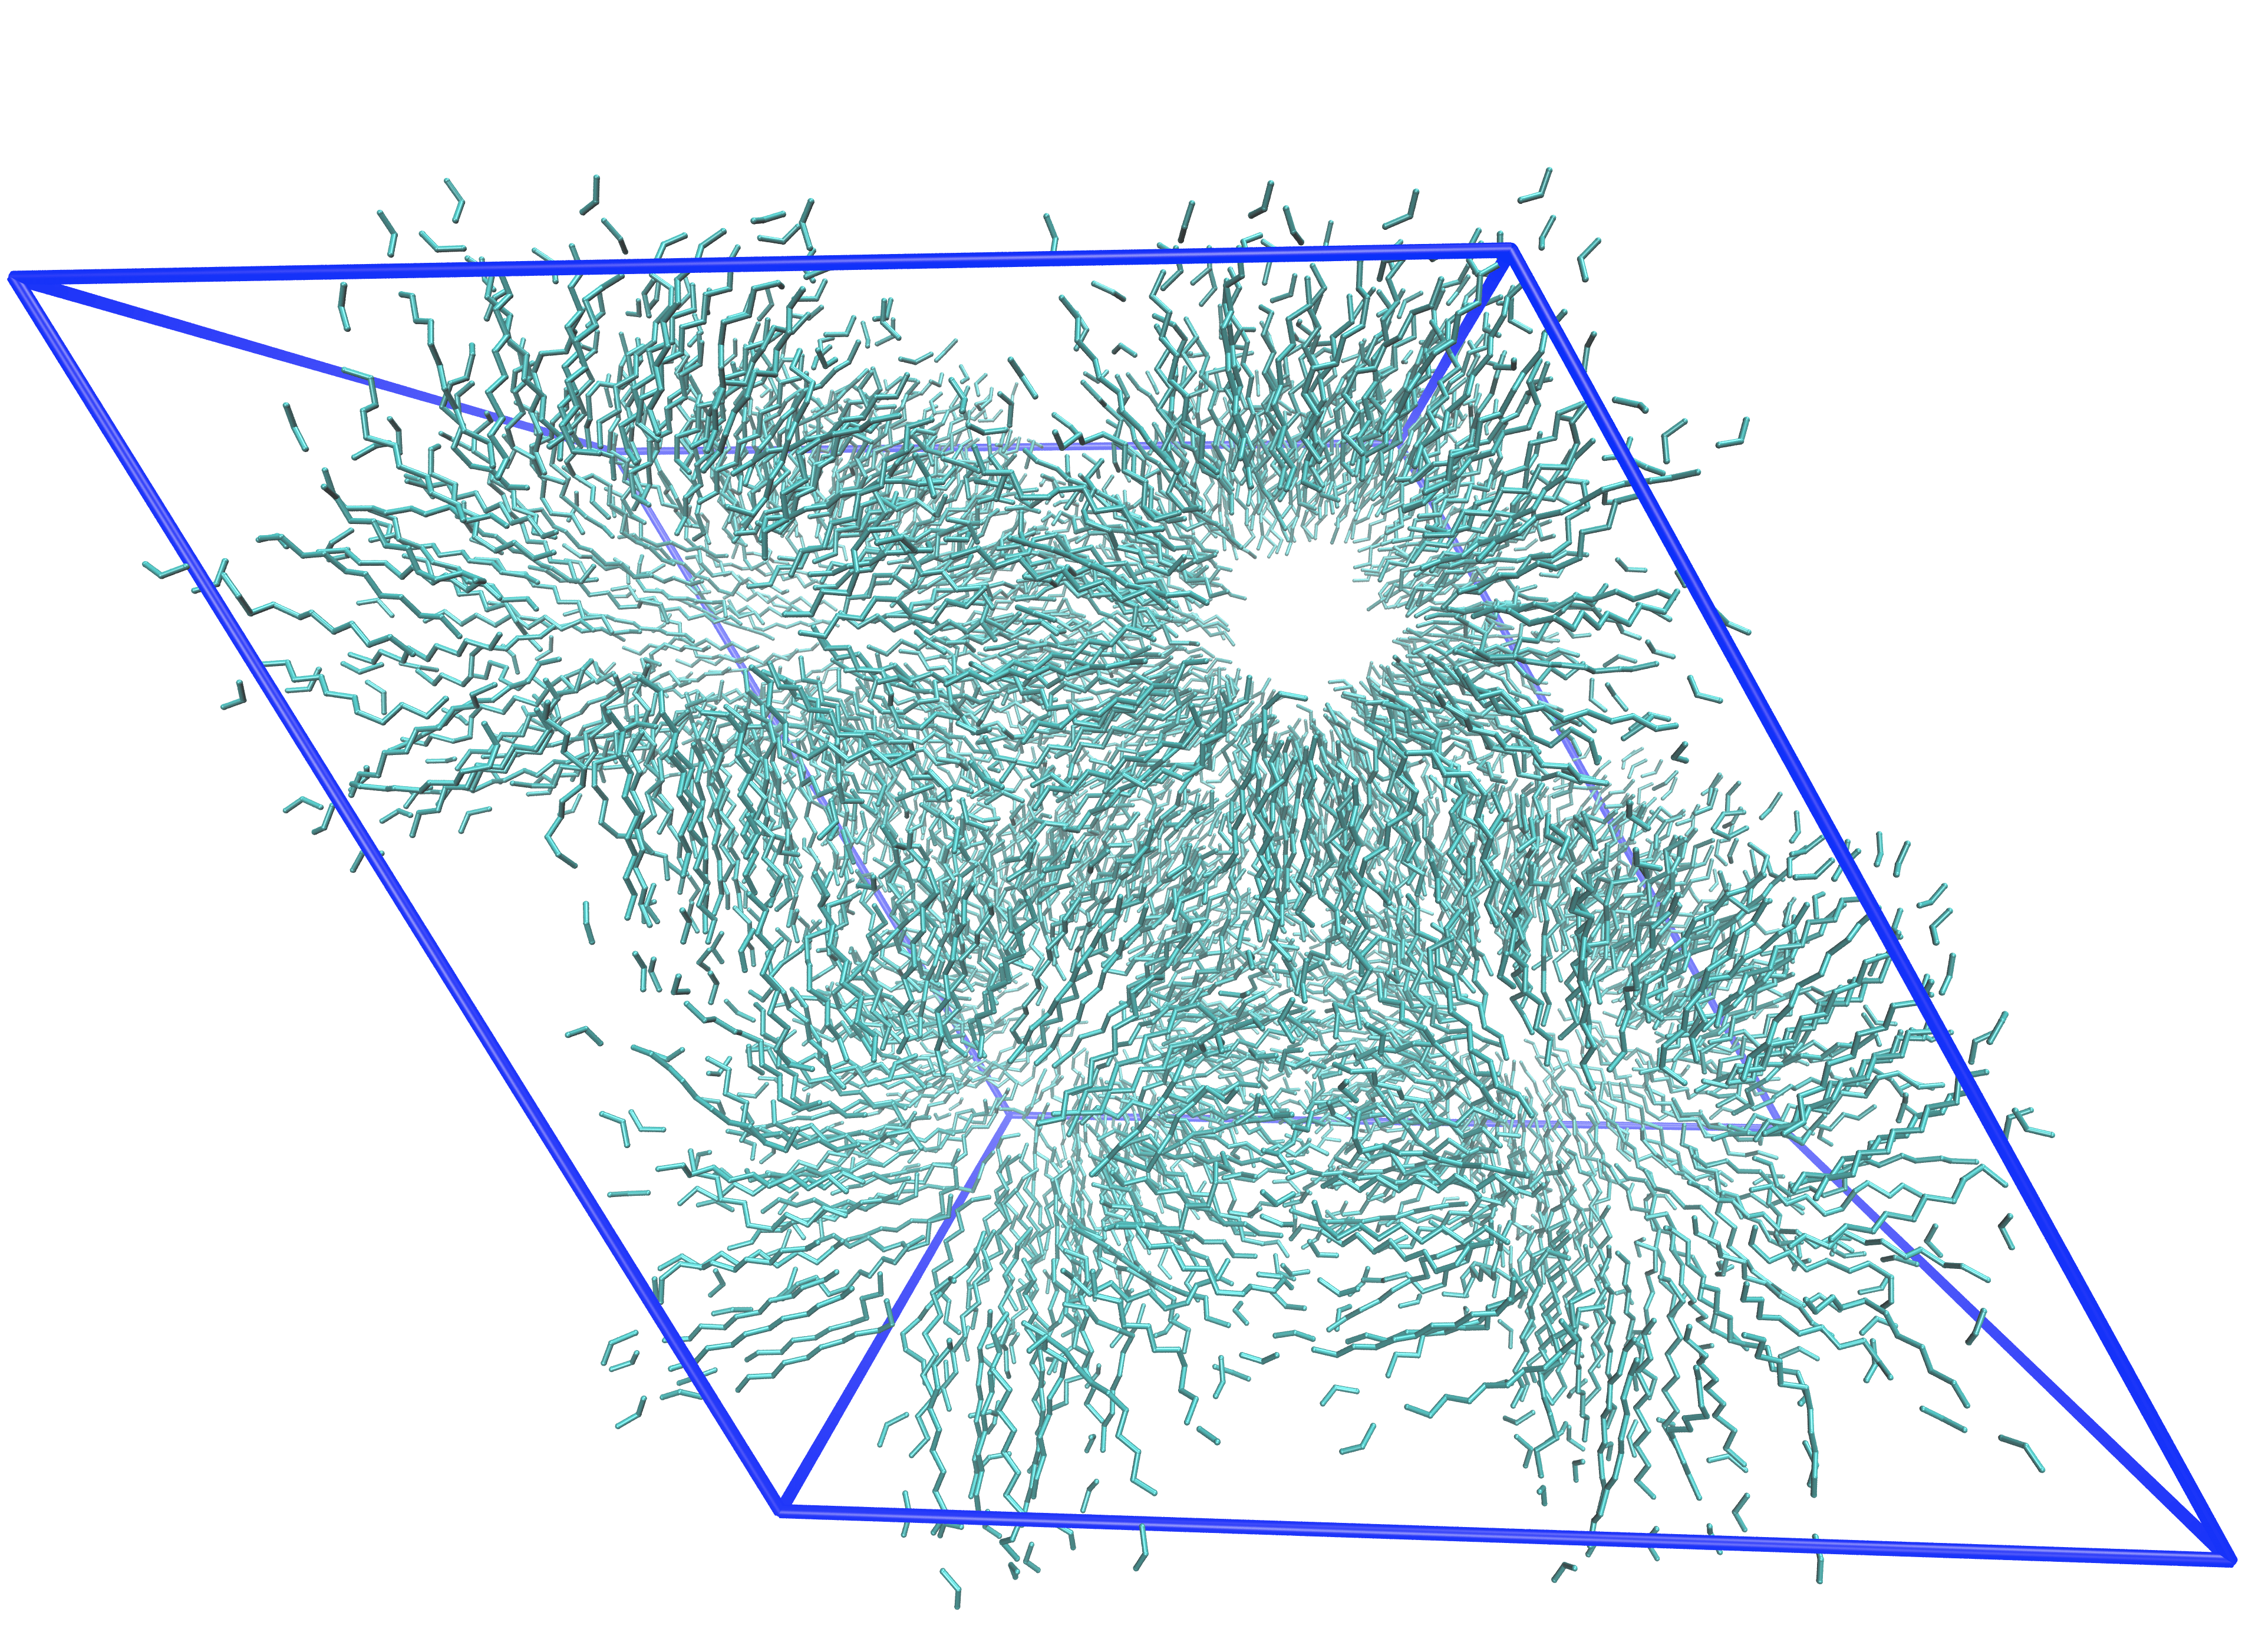
\includegraphics[width=\textwidth,scale=2]{tails_topview.png}
%                \caption{}\label{fig:tails_topview}
%        \end{subfigure}
%        \begin{subfigure}{0.45\textwidth}
%                \centering
%                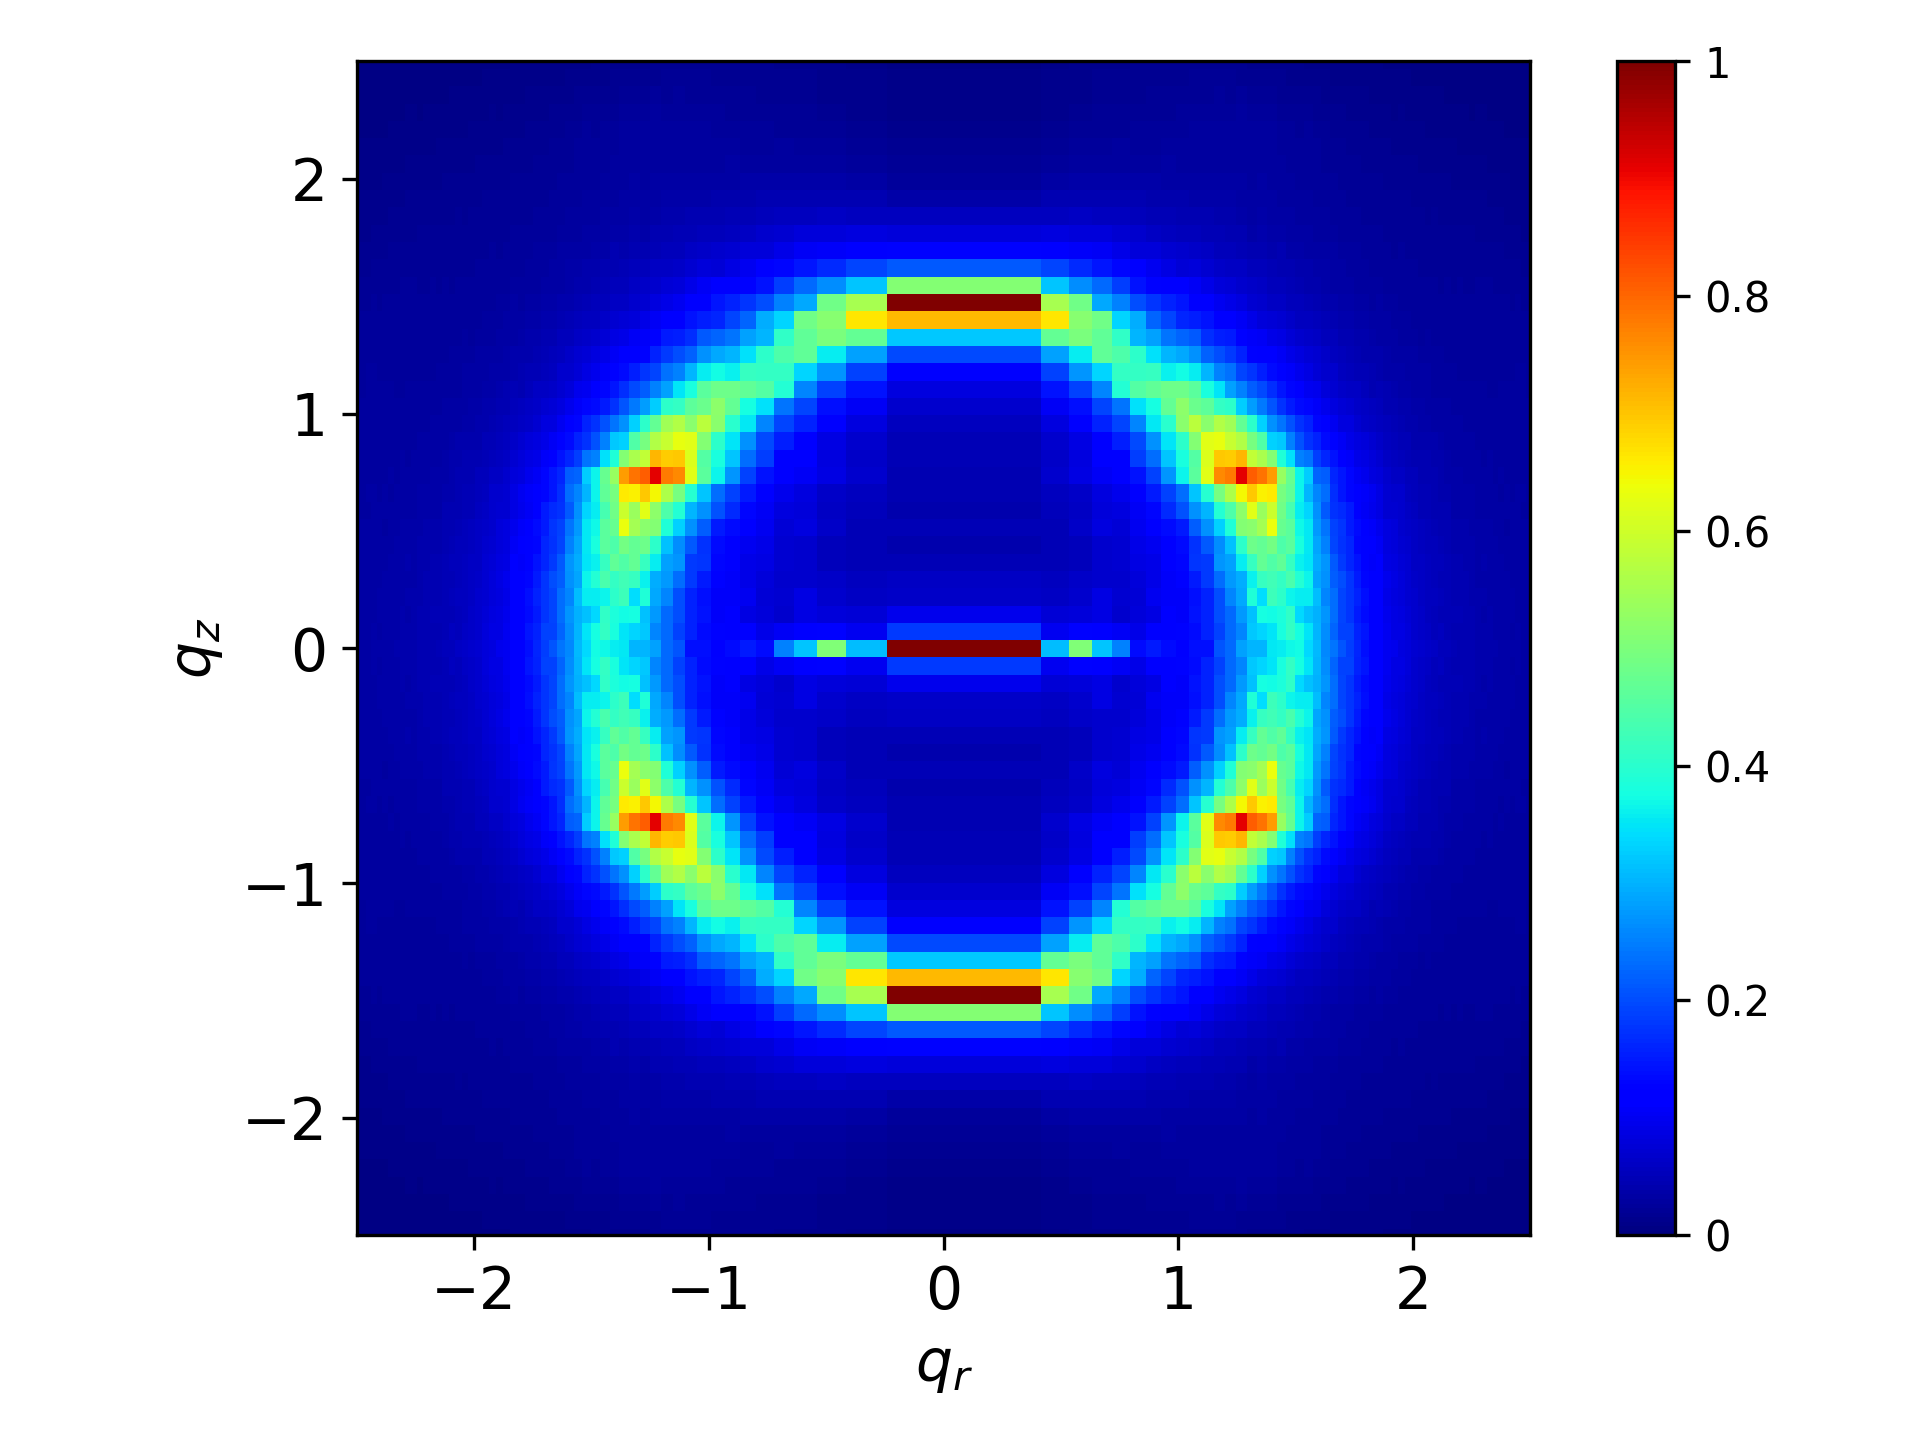
\includegraphics[width=\textwidth]{tails_rzplot.png}
%                \caption{}\label{fig:tails_rzplot}
%        \end{subfigure}
%        \begin{subfigure}{0.45\textwidth}
                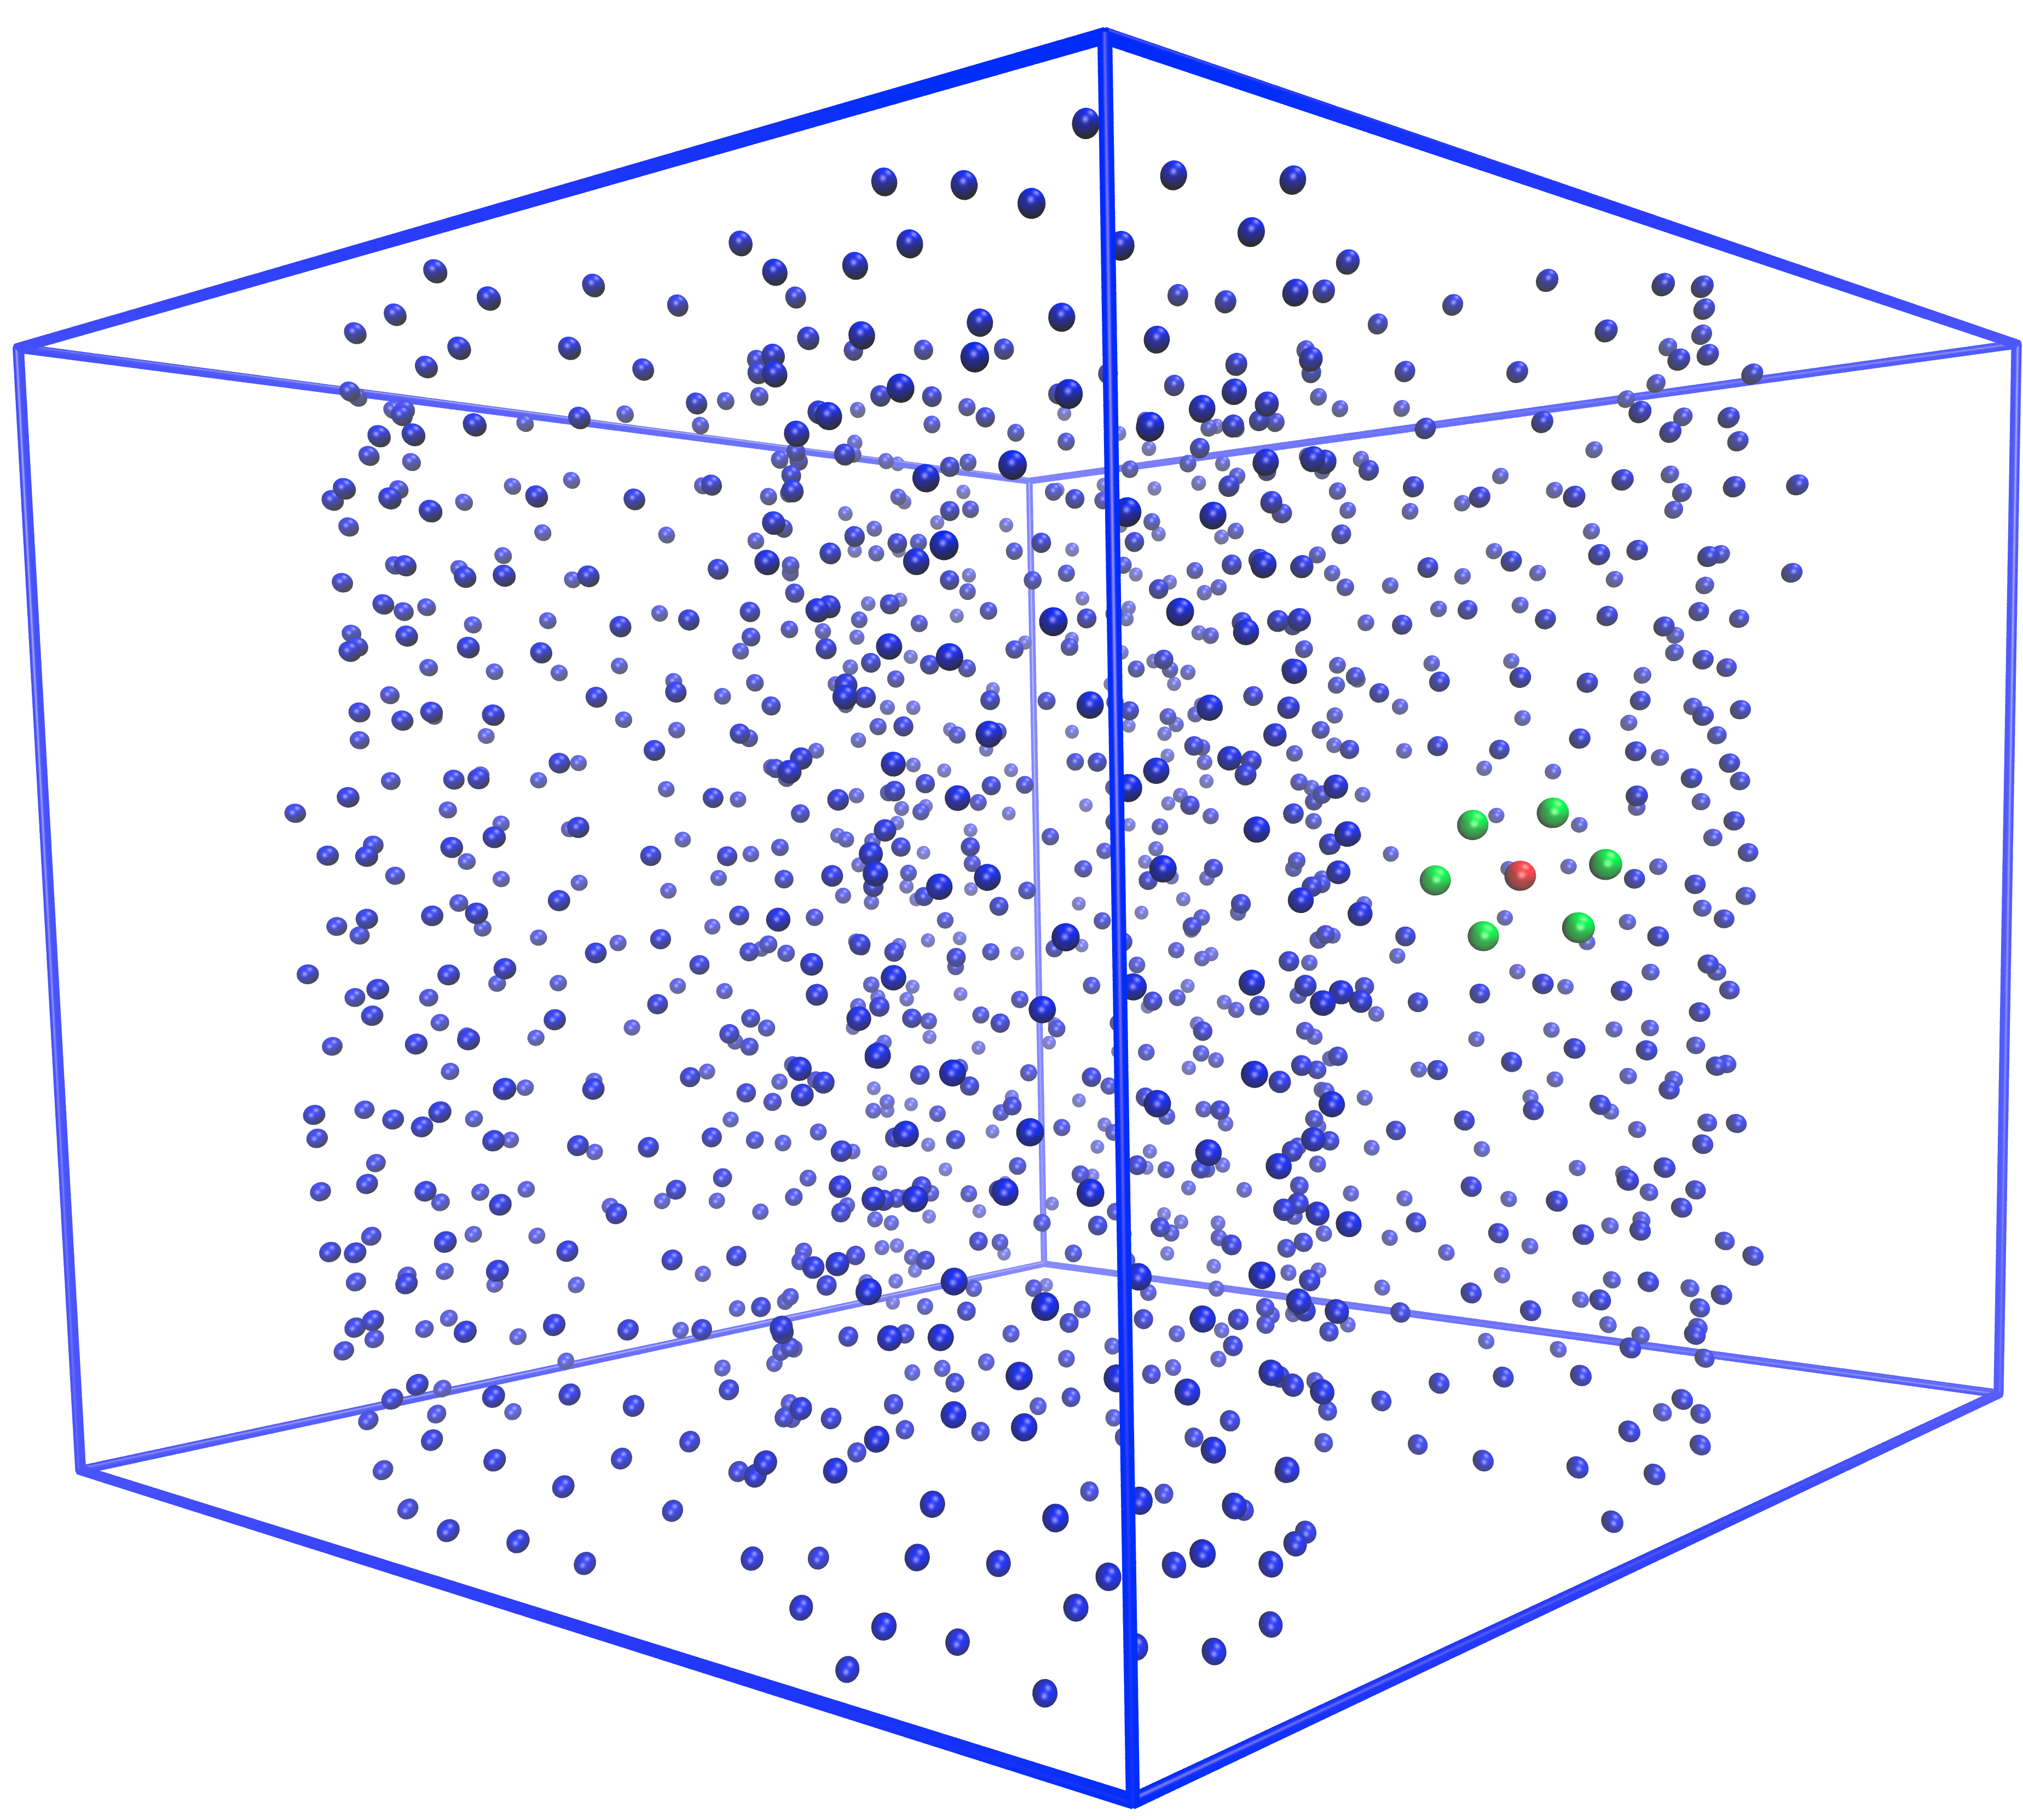
\includegraphics[width=0.5\textwidth]{centroids_box.png}
		\caption{Monomer tails pack together hexagonally. The centroid
			of each tail is visualized as a blue sphere. The centroids are calculated based
			on the red atoms in Figure~\ref{fig:monomer_color_coded}. The red sphere
			highlights an example of an alkane tail centroid with its nearest neighbors
			(green spheres) surrounding it in a hexagonal pattern.}\label{fig:centroids}
%        \end{subfigure}
%        \begin{subfigure}{0.45\textwidth}
%                \centering
%                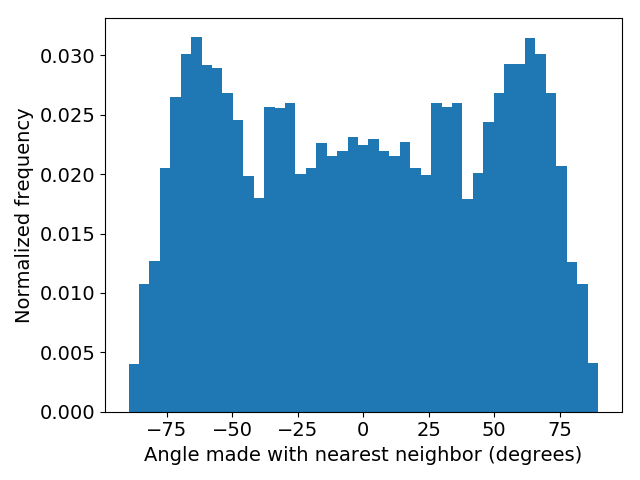
\includegraphics[width=\textwidth]{angles_traj_layered.png}
%                \caption{}\label{fig:angle_distribution}
%        \end{subfigure}
%        \caption{(a) The trajectory can be stripped of all atoms except carbon
%        atoms in monomer tails. (b) Simulated diffraction of the tail-only trajectory
%        still gives rise to R-spots. (c) Finding the center of mass and visualizing
%        their coordinates reveals the hexagonal-like packing of the tails. (d) The
%        distribution created by measuring the angle between each centroid (e.g. red
%        in (c)) and its neareset neighbors (e.g. green in (c)) with respect to the xy
%        plane has distinct spikes near 30\degree, which is consistent with the location
%        of R-spots}\label{fig:tail_packing}
  \end{figure}

  \begin{figure}
	\centering
	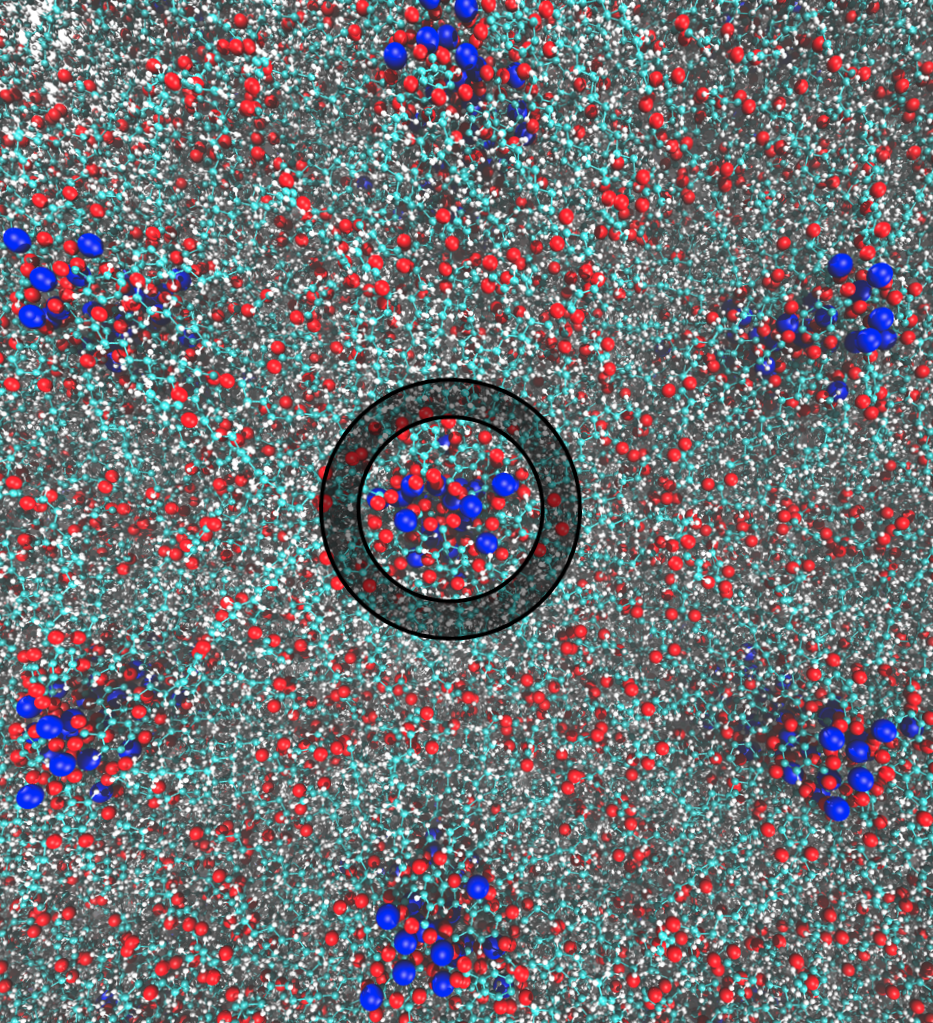
\includegraphics[width=0.75\linewidth]{radial_distribution_annulus.png}
	\caption{Looking down onto the plane of membrane, this diagram
		illustrates how we calculated radial distribution
		functions. We binned the radial distance of all atoms in 
                chosen groups from pore centers. The pore centers are 
                defined as the average coordinates of sodium ions in each
                pore. The bins are defined by the annulus bounded by concentric
		circles centered at the pore centers, as shown. To normalize, we
		divide the count of atoms within the bin annulus by the volume of
                the annulus where the volume is the area of the annulus times the
                height of the membrane in the z-direction.}~\label{fig:rdf_diagram}
  \end{figure}

  \begin{figure}
  \centering
        \begin{subfigure}{0.45\textwidth}
                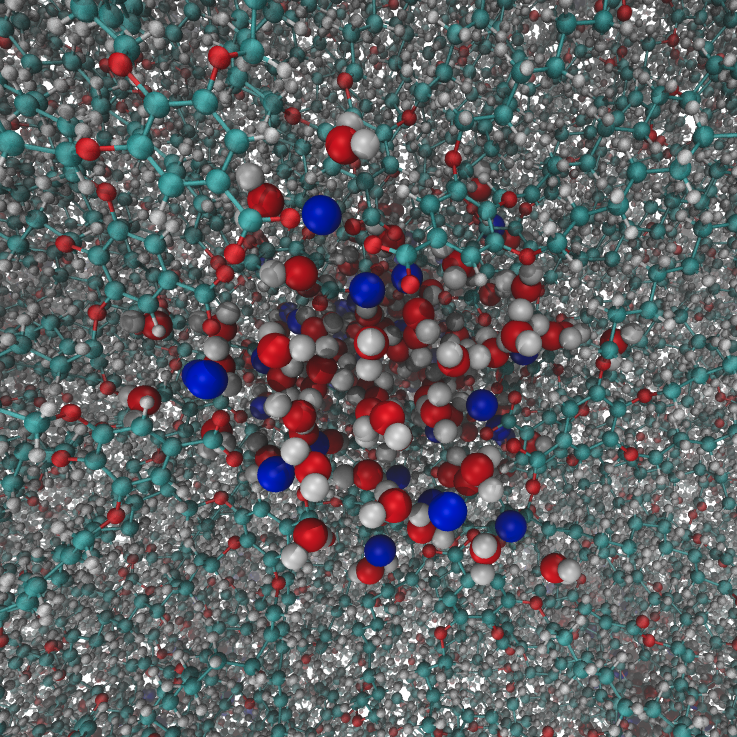
\includegraphics[width=\textwidth]{water_filled_pore.png}
                \caption{}\label{fig:water_filled_pores}
        \end{subfigure}
        \begin{subfigure}{0.45\textwidth}
                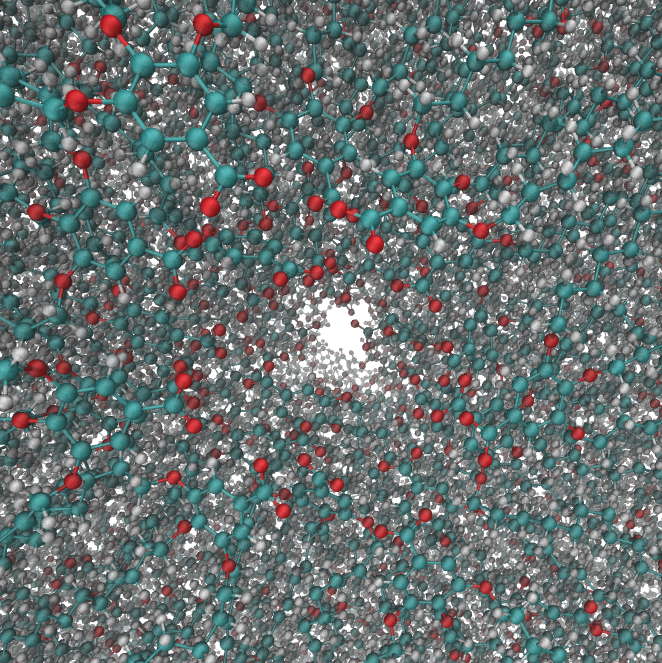
\includegraphics[width=\textwidth]{water_removed.png}
                \caption{}\label{fig:water_removed}
        \end{subfigure}
  \caption{(a) Pores built in the parallel displaced configuration with 5
	  monomers per layer are filled with 5 wt\% water. (b) The same system is
	  visualized with water molecules and sodium ions removed. Head groups vacate the
	  pore region leaving an aqeuous solution of water and sodium ions.}\label{fig:water_pores}
  \end{figure}

  \noindent
  \begingroup
        \fontsize{14pt}{14pt}\selectfont
        \textbf{Crosslinking Mechanism}
  \endgroup

  \vspace{1em}
  Crosslinking of the the monomer Na-GA3C11 occurs by a UV initiated free
  radical polymerization (Figure~\ref{fig:xlink_mech}).  Head-to-tail addition
  takes place between terminal vinyl groups on each of the monomer tails.  We
  only considered head-to-tail addition since it is the dominant propagation mode
  in the real system.   

  \begin{figure}
  \centering
  \includegraphics[width=\textwidth]{Crosslink_mechanism.eps}
  \caption{Terminal vinyl groups present on each monomer tail react with free
	  radical initiators to create monomers with terminal vinyl radicals.  Vinyl
	  radicals react with the vinyl groups of other monomers in to propagate
	  crosslinking.}\label{fig:xlink_mech}
  \end{figure}

\clearpage
\bibliography{llc}
\end{document}
